\RequirePackage[l2tabu,orthodox]{nag}

% TODO: decide if one-sided/two-sided
%\documentclass[headsepline,footsepline,footinclude=false,fontsize=11pt,paper=a4,listof=totoc,bibliography=totoc,BCOR=12mm,DIV=12]{scrbook} % two-sided
\documentclass[headsepline,footsepline,footinclude=false,oneside,fontsize=11pt,paper=a4,listof=totoc,bibliography=totoc]{scrbook} % one-sided

% TODO: change citation style in settings
\PassOptionsToPackage{table,svgnames,dvipsnames}{xcolor}

\usepackage[utf8]{inputenc}
\usepackage[T1]{fontenc}
\usepackage[sc]{mathpazo}
\usepackage[ngerman,american]{babel}
\usepackage[autostyle]{csquotes}
\usepackage[%
  backend=biber,
  url=false,
  style=alphabetic,
  maxnames=4,
  minnames=3,
  maxbibnames=99,
  giveninits,
  uniquename=init]{biblatex} % TODO: adapt citation style
\usepackage{graphicx}
\usepackage{subcaption}
\usepackage{scrhack} % necessary for listings package
\usepackage{listings}
\usepackage{lstautogobble}
\usepackage{tikz}
\usepackage{pgfplots}
\usepackage{pgfplotstable}
\usepackage{booktabs}
\usepackage[final]{microtype}
\usepackage{caption}
\usepackage[hidelinks]{hyperref} % hidelinks removes colored boxes around references and links
\usepackage{textgreek}

\bibliography{bibliography}

\setkomafont{disposition}{\normalfont\bfseries} % use serif font for headings
\linespread{1.05} % adjust line spread for mathpazo font

% Add table of contents to PDF bookmarks
\BeforeTOCHead[toc]{{\cleardoublepage\pdfbookmark[0]{\contentsname}{toc}}}

% Define TUM corporate design colors
% Taken from http://portal.mytum.de/corporatedesign/index_print/vorlagen/index_farben
\definecolor{TUMBlue}{HTML}{0065BD}
\definecolor{TUMSecondaryBlue}{HTML}{005293}
\definecolor{TUMSecondaryBlue2}{HTML}{003359}
\definecolor{TUMBlack}{HTML}{000000}
\definecolor{TUMWhite}{HTML}{FFFFFF}
\definecolor{TUMDarkGray}{HTML}{333333}
\definecolor{TUMGray}{HTML}{808080}
\definecolor{TUMLightGray}{HTML}{CCCCC6}
\definecolor{TUMAccentGray}{HTML}{DAD7CB}
\definecolor{TUMAccentOrange}{HTML}{E37222}
\definecolor{TUMAccentGreen}{HTML}{A2AD00}
\definecolor{TUMAccentLightBlue}{HTML}{98C6EA}
\definecolor{TUMAccentBlue}{HTML}{64A0C8}

% Settings for pgfplots
\pgfplotsset{compat=newest}
\pgfplotsset{
  % For available color names, see http://www.latextemplates.com/svgnames-colors
  cycle list={TUMBlue\\TUMAccentOrange\\TUMAccentGreen\\TUMSecondaryBlue2\\TUMDarkGray\\},
}

% Settings for lstlistings
\lstset{%
  basicstyle=\ttfamily,
  columns=fullflexible,
  autogobble,
  keywordstyle=\bfseries\color{TUMBlue},
  stringstyle=\color{TUMAccentGreen}
}


% TODO: change thesis information
\newcommand*{\getUniversity}{Technische Universität München}
\newcommand*{\getFaculty}{Department of Informatics}
\newcommand*{\getTitle}{Thesis title}
\newcommand*{\getTitleGer}{Titel der Abschlussarbeit}
\newcommand*{\getAuthor}{Author}
\newcommand*{\getDoctype}{Thesis type (Bachelor's Thesis in Informatics, Master's Thesis in Robotics, \ldots)}
\newcommand*{\getSupervisor}{Supervisor}
\newcommand*{\getAdvisor}{Advisor}
\newcommand*{\getSubmissionDate}{Submission date}
\newcommand*{\getSubmissionLocation}{Munich}

\begin{document}

\setcounter{secnumdepth}{4} % how many sectioning levels to assign numbers to
\setcounter{tocdepth}{4}    % how many sectioning levels to show in ToC


% Set page numbering to avoid "destination with the same identifier has been already used" warning for cover page.
% (see https://en.wikibooks.org/wiki/LaTeX/Hyperlinks#Problems_with_Links_and_Pages).
\pagenumbering{alph}
\begin{titlepage}
  % HACK for two-sided documents: ignore binding correction for cover page.
  % Adapted from Markus Kohm's KOMA-Script titlepage=firstiscover handling.
  % See http://mirrors.ctan.org/macros/latex/contrib/koma-script/scrkernel-title.dtx,
  % \maketitle macro.
  \oddsidemargin=\evensidemargin\relax
  \textwidth=\dimexpr\paperwidth-2\evensidemargin-2in\relax
  \hsize=\textwidth\relax

  \centering

  \IfFileExists{logos/tum.pdf}{%
    \includegraphics[height=20mm]{logos/tum.pdf}
  }{%
    \vspace*{20mm}
  }

  \vspace{5mm}
  {\huge\MakeUppercase{\getFaculty{}}}\\

  \vspace{5mm}
  {\large\MakeUppercase{\getUniversity{}}}\\

  \vspace{20mm}
  {\Large \getDoctype{}}

  \vspace{15mm}
  {\huge\bfseries \getTitle{}}

  \vspace{15mm}
  {\LARGE \getAuthor{}}

  \IfFileExists{logos/faculty.pdf}{%
    \vfill{}
    \includegraphics[height=20mm]{logos/faculty.pdf}
  }{}
\end{titlepage}


\frontmatter{}

\begin{titlepage}
  \centering

  \IfFileExists{logos/tum.pdf}{%
    \includegraphics[height=20mm]{logos/tum.pdf}
  }{%
    \vspace*{20mm}
  }

  \vspace{5mm}
  {\huge\MakeUppercase{\getFaculty{}}}\\

  \vspace{5mm}
  {\large\MakeUppercase{\getUniversity{}}}\\

  \vspace{20mm}
  {\Large \getDoctype{}}

  \vspace{15mm}
  {\huge\bfseries \getTitle{}}

  \vspace{10mm}
  {\huge\bfseries \foreignlanguage{ngerman}{\getTitleGer{}}}

  \vspace{15mm}
  \begin{tabular}{l l}
    Author:          & \getAuthor{} \\
    Supervisor:      & \getSupervisor{} \\
    Advisor:         & \getAdvisor{} \\
    Submission Date: & \getSubmissionDate{} \\
  \end{tabular}

  \IfFileExists{logos/faculty.pdf}{%
    \vfill{}
    \includegraphics[height=20mm]{logos/faculty.pdf}
  }{}
\end{titlepage}

\thispagestyle{empty}
\vspace*{0.8\textheight}
\noindent
I confirm that this \MakeLowercase{\getDoctype{}} is my own work and I have documented all sources and material used.

\vspace{15mm}
\noindent
\getSubmissionLocation{}, \getSubmissionDate{} \hspace{50mm} \getAuthor{}

\cleardoublepage{}

\addcontentsline{toc}{chapter}{Acknowledgments}
\thispagestyle{empty}

\vspace*{20mm}

\begin{center}
{\usekomafont{section} Acknowledgments}
\end{center}

\vspace{10mm}

%TODO: Acknowledgments

\cleardoublepage{}

\chapter{\abstractname}

%TODO: Abstract



\microtypesetup{protrusion=false}
\tableofcontents{}
\microtypesetup{protrusion=true}

\mainmatter{}

% !TeX root = ../main.tex
% Add the above to each chapter to make compiling the PDF easier in some editors.

\chapter{Introduction}\label{chapter:introduction}
Some Introduction will go here
\section{Problem and solution overview}

\subsection{Motivation}
In Augmented Reality or Mixed Reality, tracking is one of the most important as well as challenging tasks. Tracking means to detect the position and orientation of an object to a coordinate system in real-time. Tracking has to be very accurate, precise and robust otherwise misalignment will occur between the virtual and real objects in the frame which makes the experience much less pleasant to the user. In the sector of medical augmented reality, the situation can be severe.

There are many methods for tracking an object. We can track an object by multiple camera setup or use mechanical sensors such as Inertial Measurement Unit (IMU) or we can use hybrid approaches combining both camera and mechanical sensors.

The problem with tracking objects with cameras or hybrid systems is that it needs an external camera setup which is not portable and the setup can be problematic to the user. In order to track objects without the camera, we use a mechanical sensor such as IMU, which is portable and embedded in the Head Mounted Display (HMD). Here sensor fusion comes handy. Sensor fusion is a technic for combining sensory data from multiple sensors output which gives better results for tracking. In the case of IMU sensory data, prior work[] shows that increasing the number of IMU tends to provide better accuracy.

\subsection{Goals}
Our goal is to develop a deep learning model primarily with Convolutional Nural Network (CNN) and Dense Network to fuse multiple IMU data in a simulated environment. We will use many combinations of several IMUs and different CNN networks to predict the position and orientation of an object in a simulated environment and compare the results with other Deep Learning technics such as Recurrent Neural Network (RNN). We will take the combination which provides the best accuracy in the simulated environment and apply that model in a real-world scenario to test its accuracy to predict object pos.

Acceleration values from an IMU are well known to be highly unstable and there could be misalignment between axes. Using Deep Learning, we aim to achieve a stable and reliable position and orientation transformation without any camera, sensor calibration, registration, and prior error correction.


\section{Structure of the Thesis}

This document is divided in five chapters. In the second chapter, the necessary
theoretical background is presented, whereas third chapter shows the structural
solution and implementation. Chapter four introduces the obtained results and
pertinent analysis, while the conclusions and proposed future work are summarized
in chapter five. Afterwards, references and relevant bibliography are presented and
the document ends with Appendices where outcomes of every experiment are detailed
in their plots.

% !TeX root = ../main.tex
% Add the above to each chapter to make compiling the PDF easier in some editors.

\chapter{Background}\label{chapter:background}

\section{Sensor}

Our modern world us infused with sensors. We use sensors in everyday life concisely or subconsciously. From our smartphone, cars to the state of the art medical equipment, mars roves has a variety of uses of sensors. Although when the term sensor comes up we think about mostly mechanical sensors, such as touchscreen in our smartphone or the fire detection sensor, sensors can be not only mechanical but also chemical, bio, and other variety of types.

These sensors are collecting data every moment in our modern world. For example, our buses, trains, planes, and ships are using GPS to navigate around the world. We are using our smartphone which has a variety of sensors working together like the camera, touch sensors, gyro, GPS, and proximity sensor. They are working continuously in the background and processing data to make our life a  little bit easier. Now we can sense and track out heartbeat just using a wristwatch.

The use of smart sensors in our homes, offices, shopping malls, cars is getting bigger and bigger nowadays. All modern means of transport such as cars, buses, trains are using sensors to create a more comfortable transport experience. For instance, proximity sensors for better parking experience, crash prevention. If we talk about air transportation, the impact of sensors is even more important and critical for instance temperature, air pressure sensors. A single failure of any of these sensors could lead to deadly outcomes with fatality. The list goes on when it comes to the use of sensors and their impacts on our life

n the broadest definition, a sensor is a device that can  monitor the environment that its designed for. A sensor is a device or an integrated system of devices that senses and responds to certain types of environmental inputs. Light, heat, movement, moisture, pressure, or any of a number of other environmental phenomena could be the specific input. The output is usually a signal converted for reading or continuing processing to a human-readable display at the point of the sensor or electronically transmitted over a network. Due to the different needs, the properties of sensors were changed a lot over time. The need enabled intelligent and intelligent sensors to be created. The advent of intelligent sensors led to the development of microcontrollers used everywhere. The smart sensors have allowed us to interface with other devices and make them work together as one device.


\subsection{Sensor Types}

As we mentioned before, sensors can be many types, It can be categorized depending on their purpose or depending on how they are made. There are various sensor classifications created by different writers and specialists. An expert in the subject can already use the following sensor classification, but it is an extremely simple sensor classification. They are divided into active and passive in the first classification of the sensors. Active sensors are those that require a power signal or an external excitation signal. On the other hand, passive sensors do not require an external power signal and generate an output response directly. Analog and optical sensors are the final grouping of the sensors. Analog capabilities generate an analog output.

We have a long list of sensors, which we use in our everyday work. If we want to speak briefly about them, we can hardly cover each sensor. We will discuss a few of them which is somewhat related to our work. The sensor mention below are regardless of their classes, they are a mix of digital, analog, active sensors.

\subsubsection{Temperature sensors or thermal sensors}

This system collects temperature information from a system and transforms it into a way that another system or individual can understand. Mercury in a glass thermometer is the simplest example of a temperature sensor. Mercury expands in the glass and contracts to rely on temperature changes. The external temperature is the source factor for measuring the temperature. In order to calculate the temperature, the spectator measures the location of mercury. Two basic temperature sensors are available:

\begin{figure}[h]
  \centering
    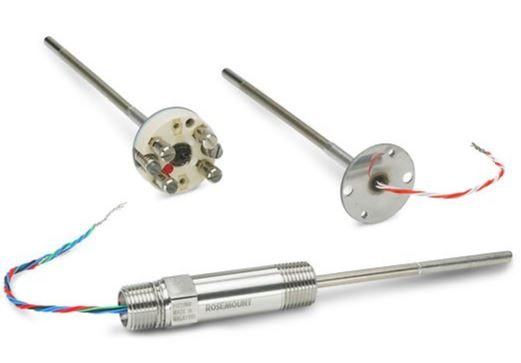
\includegraphics[width=0.8\linewidth]{figures/tempSensor.jpg}
    \caption{A typical temperature sensor.}
    \source {emerson.com}
\label{fig:tempSensor}
\end{figure}


\begin{itemize}
 \item Contact sensors – This type of sensor requires physical direct contact with the sensed object or media. They monitor solids, liquids, and gas temperatures across a broad range of temperatures.
 \item  Non-contact Sensors – No physical contact with the object or the media is required for this type of sensor. They monitor non-reflective solids and liquids, but because of natural transparency, they are not useful for gasses. These sensors use the Law of Plank for temperature calculation. This law covers heat radiated from the heat source for temperature measurements.

\end{itemize}


\subsubsection{Sonar sensors}


Sonar sensor: As the name suggests, the Sonar sensor also known as Ultrasonic sensor works based on an ultrasonic pulse time calculation to measure distance.


\begin{figure}[h]
  \centering
    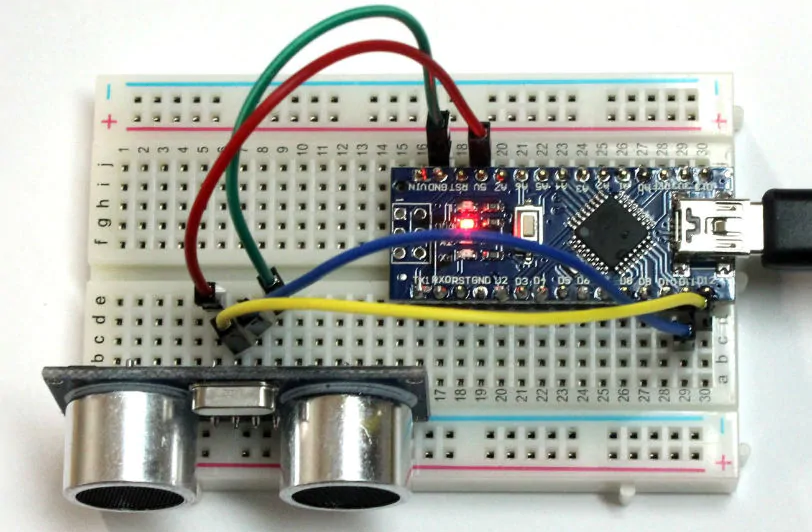
\includegraphics[width=\linewidth]{figures/sonarSensor.png}
    \caption{A sonar sensor combined with microcontroller}
    \source {arrow.com}
\label{fig:sonarSensor}
\end{figure}


To measure the specific distance from the sensor, this can be calculated based on this formula \cite{sonar1}:

Distance = 1/2 T x C 


where T is time and C is the spped of sound in specific temparatuer of earth environment. At 20$^{\circ}$ C (68$^{\circ}$ F), the speed of sound is 343 meters/second (1125 feet/second), but this varies depending on temperature and humidity.


\subsubsection{IR Sensors}

These types of sensors sense the infrared light. In general, all objects on the infrared ( IR ) spectrum emit thermal radiation. That kind of radiation that is not visible to the human eye is measured by the infrared sensor. The biggest advantage of the IR sensor is that it uses very cheap and available and very easy to use. One of the major drawbacks of these sensors is that it pruned to background noise.

\begin{figure}[h]
  \centering
    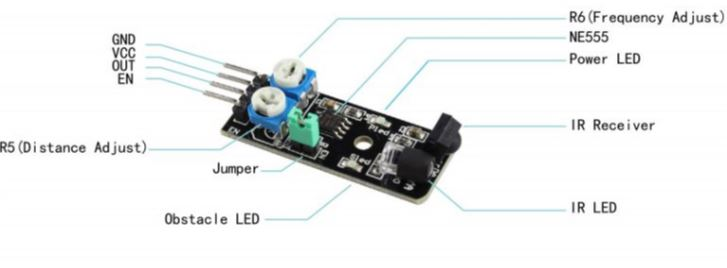
\includegraphics[width=\linewidth]{figures/irSensor.jpg}
    \caption{An IR sensor architecture}
    \source {ram-e-shop.com}
\label{fig:irSensor}
\end{figure}


The working of IR sensor and sonar sensor is similar, where the sonar sensor emits soundwave and have a receiver for the sound wave the IR use infrared light instead of sound. 

\begin{figure}[h]
  \centering
    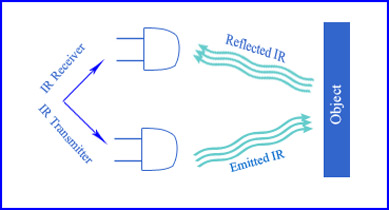
\includegraphics[width=0.5\linewidth]{figures/irSensorWork.jpg}
    \caption{Working principal of an IR sensor}
    \source {engineersgarage.com}
\label{fig:irSensorWork }
\end{figure}


\subsubsection{UV Sensors}

Such sensors measure the intensity or strength of the UV radiation incident. It has a longer wavelength than x-rays but is also shorter than the visible radiation. For robust ultraviolet sensing, an active material called polycrystalline diamond is used. UV sensors can detect exposure to ultraviolet radiation from the environment.


\begin{figure}[h]
  \centering
    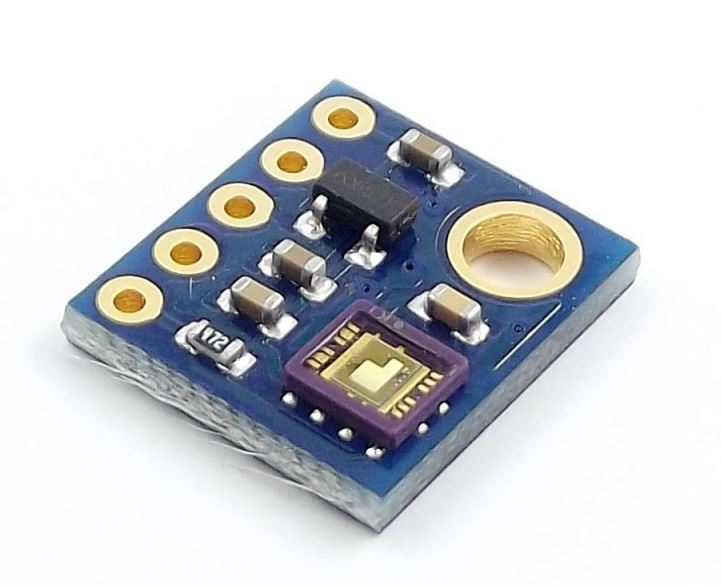
\includegraphics[width=0.5\linewidth]{figures/uvSensor.jpg}
    \caption{UV sensor}
    \source {roboticsbd.com}
\label{fig:uvSensor }
\end{figure}


The UV sensor recognizes one energy signal type and transmits different energy signals. They are directed to an electric meter to observe and record these output signals. The output signals are transmitted for the generation of graphs and reports to a software-based computer through an analog-to-digital converter ( ADC).


\subsubsection{Touch Sensor}

A touch sensor functions as a variable resistor according to the position of the touch. As seen in figure \ref{touchSensorWork}

\begin{figure}[h]
  \centering
    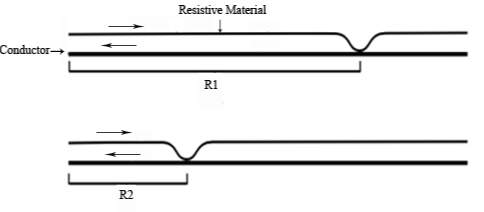
\includegraphics[width=0.5\linewidth]{figures/touchSensorWork.png}
    \caption{Working mecanism of a touch sensor}
\label{fig:touchSensorWork }
\end{figure}

A touch sensor made of a substance that is absolutely conductive such as copper Isolated material for the spacing of foam or plastic or material which is partly conductive.
The way the touch sensor works is that the surface is partly conductive and opposes the present flow. The key concept of the linear position sensor is that when the length of this material, to be traveled by the current, is greater, the current flow is contrasted. The resistance of the material is therefore varied by adjusting the location at which it comprises the substance that is completely conductive.

\subsubsection{Global Positioning System (GPS) sensor}

We use the GPS sensor almost every day in our life, mostly via our phone or in our car, the GPS sensor is used to navigate around the world.

A minimum of 24 operational satellites orbit over 12,000 kilometers above ground at any given time. The locations of the satellites will always include up to 12 satellites in the sky above your location. The primary function of the 12 visible satellites is to relay radio frequency (1.1-1.5 GHz) information back to earth. A soil-based receiver or GPS module may measure its location and time with this information and other mathematical details. \cite{misra2006globa}



\subsubsection{LiDAR}

Lidar is an analogy for "light detection and ranging." The device uses eye-safe laser beams to produce a 3D view of the surroundings being scanned.


\begin{figure}[h]
  \centering
    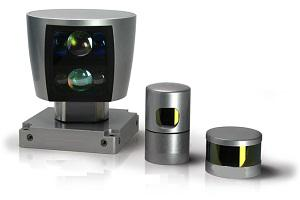
\includegraphics[width=0.5\linewidth]{figures/lidarSensor.jpg}
    \caption{A Lidar device used for automotive}
    \source {Automotive Lidar Sensor Market 2017 - Leddar, Quanergy}
\label{fig:lidarSensor}
\end{figure}


A typical lidar sensor absorbs the ambient atmosphere with pulsed light waves. Such pulses rebound and come back to the sensor. To calculate the distances traveled, the sensor takes time for every pulse to return to the sensor. This procedure is repeated millions of times per second and creates a precise 3D environmental map in real-time. This chart can be used for secure surfing by an onboard computer.
Lidar is mostly used for advance autonomous systems to measure its surrounding environment.


\subsubsection{Gyroscope sensor}


A device that senses angular velocity is gyro sensors, also known as angular rate sensors or angular velocity sensors.  Gyroscopes in consumer électronics were not only found in compasses, ships, computer pointing instruments, etc.

\begin{figure}[h]
  \centering
    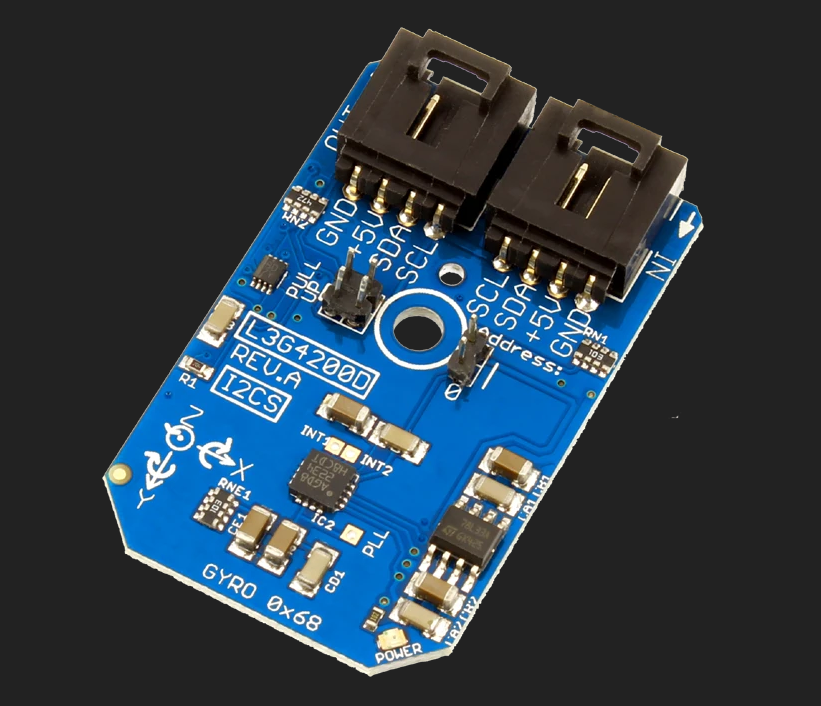
\includegraphics[width=0.5\linewidth]{figures/gyroSensor.png}
    \caption{An MMSE gyroscope}
    \source {controleverything.com}
\label{fig:gyroSensor}
\end{figure}

Since the gyroscope allows orientation and rotation to be measured, designers have combined them with modern technology. The gyroscope technology has made it possible to detect the movement inside a 3D world more reliably than the previous lone accelerometer on most smartphones. Gyroscopes are also paired with accelerometers for better direction and motion sensing in consumer electronics. The gyroscopes inside smartphones don't have wheels and gimbals such as the conventional mechanical ones in an old aircraft, they are MEMS (Micro-Electro-Mechanical Systems)  gyroscopes instead.



\subsubsection{Accelerometer sensor}



It can be used for the measurement of the acceleration exerted on the sensor, as its name implies. The acceleration is usually performed in two or three components of the axis-vector, which make up the acceleration. \cite{FERNANDEZ20138} There are a few uses of Accelerometers, remote controls for videos, smartphones, etc. Accelerometer usually combined with a Gyroscope for better sensing. Accelerometers give us two data types: Static force used on the sensor due to gravity detection in the direction of orientation and  Sensor strength, acceleration to motion, force detection

\begin{figure}[h]
  \centering
    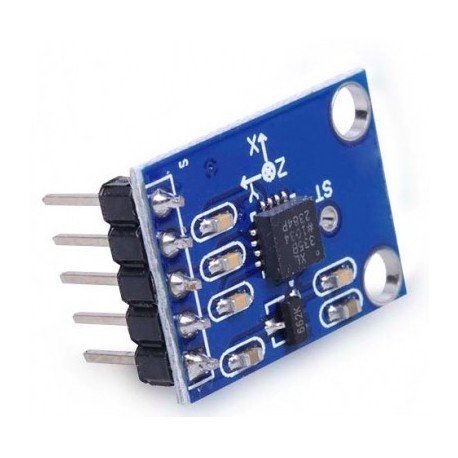
\includegraphics[width=0.5\linewidth]{figures/accSensor.jpg}
    \caption{An electronic accelerometer sensor}
    \source {nuttyengineer.com}
\label{fig:accSensor}
\end{figure}



\subsubsection{Smart Sensors}

Due to the different needs, the sensor characteristics were adjusted a lot over time. The needs allowed intelligent and intelligent sensors to be developed. The IEEE 1451 standard defines smart sensors as a physical device or a combination of sensors with physical connectors for communication with processor and data network. \cite{5739775}.

Fig (smartSensorStructure) source cite [5739775]
\begin{figure}[h]
  \centering
    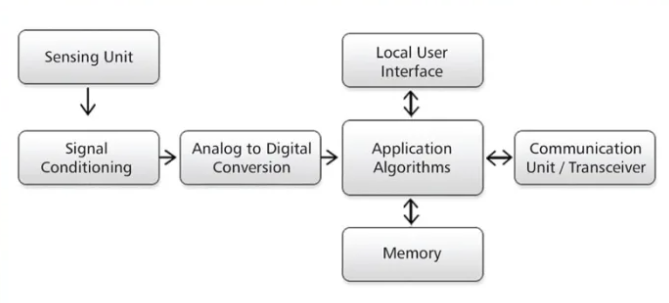
\includegraphics[width=\linewidth]{figures/smartSensorStructure.png}
    \caption{ Smart sensor building blocks }
    \source {Premier Farnell Ltd}
\label{fig:smartSensorStructure}
\end{figure}


The advent of smart sensors contributed to the development of microcontrollers used all over the world. Because of the intelligent sensors, interfacing and working with other peripherals as a single device was possible.
These smart sensors allow us to reduce data volume for communication with the main processor and made faster communication possible. It also reduced power consumption because multiple sensors are used together that use the same processing unit. The major benefit of these smart sensor is that they are typically small and very easy to integrate with other systems even with other sensors.

Here come the uses of IMU (Inertial Measurement Units). In the next section, we describe the properties of an IMU.


\subsection{IMU (Inertial Measurement Units)}
As our goal is to use IMU as our main sensor to collect data for acquiring objects position and orientation, this is our principal sensor to study. An IMU is typically a combination (Accelerometer, Gyroscope, Magnetometer) of sensors working together.
In this chapter, we will discuss the IMU, how its functions, its general structure, and the use cases.

\subsubsection{General structure}

The IMU typically consists of 3 individual sensors Accelerometer, Gyroscope, and a Magnetometer. Sometimes it comes with only an Accelerometer and Gyroscope. The Accelerometer, Gyroscope, and a Magnetometer provides the data of acceleration and velocity, orientation and angular velocity, gravitational forces respectively. This typically gives us the 9 axes of measurement on the other hand the IMU consist of only Accelerometer and Gyroscope provide 6 axes of measurement.
Early days the size of IMU was considerably larger compared to the current IMUs. Its because those are made mechanically but thanks to the MEMS or Micro-Electro-Mechanical Systems that are made possible to make these sensors electronically it's miniaturized the size considerably. \cite{MEMS}.
This helps us to integrate with other microcontrollers or microprocessors like Arduino or Raspberry Pi. Due to its miniature of size sometimes the IMUs are also known as MIMU (Miniature Inertial Measurement Units) \cite{2018233}

\begin{figure}[h]
  \centering
    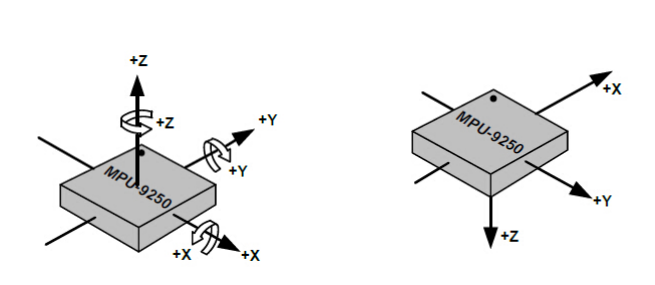
\includegraphics[width=\linewidth]{figures/imuAG.png}
    \caption{ An IMU with 6DoF workiks with a magnetometer for 9DoF }
    \source {Stanford.edu lecture 9 of EE267: Virtual Reality S2020}
\label{fig:imuAG}
\end{figure}


\subsubsection{Working principal of IMU}
The main purpose of IMU is to measure and objects pose relative to its inertial space. Acceleration and angular speed are based on inertial principles are measured.

Accelerometers calculate in a particular direction linear acceleration. An accelerometer can be also used as a downward force to measure gravity. Integrating acceleration once shows a velocity estimate, and integrating again provides you with a position estimate.


\begin{equation}
f^{b}=R^{b n}\left(a_{i i}^{n}-g^{n}\right)
\end{equation}


Although accelerometers can measure linear acceleration, they are unable to measure orientation or rotational motion. Nevertheless, gyroscopes measure angular velocities along three axes: pitch (x-axis), roll (y-axis), and yaw (z-axis). While a gyroscope does not have an initial frame of reference (like gravity), for measuring angular position, you can combine its data with data from an accelerometer. Gyroscope data output angular velocity (deg/s).

The gyroscope measures the angular velocity of the body frame with respect to the inertial frame, expressed in the body frame \cite{ROS}, denoted by $\omega $. This angular velocity can be expressed as

\begin{equation}
\tilde{\omega}=\omega+b+\eta
\end{equation}

The estimated orientation can be obtained by integrating these angular velocities. We can also use Taylor series to measure discrete-time approximation of integration

%\begin{equation}{\theta}_{\text {gyro}}^{(t)}={\theta}_{\text {gyro}}^{(t-1)}+\tilde{{\omega}} \Delta t\end{equation}

Using 3 Gyro and Accelerometer we can obtain an estimated pose of the object in 3D space.
The working principle of a single unit of IMU can be seen in the figure \ref{fig:imuWP}


\begin{figure}[h]
  \centering
    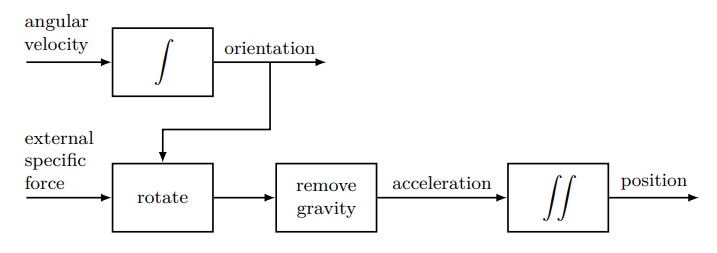
\includegraphics[width=\linewidth]{figures/imuWP.png}
    \caption{ working principle of a single unit of IMU }
    \source {Stanford.edu lecture 9 of EE267: Virtual Reality S2020}
\label{fig:imuWP}
\end{figure}







\section{Sensor fusion}

\subsection{Need of sensor fusion}

First, we have to ask our selves why we need to do sensor fusion if we can get the pose of an object from a single IMU as we can see in the calculation from the previous section {ref section}. But the real-world situation is not an ideal situation. This will only work when there is no bias and no noise but which is unrealistic in the real world. Even if the bias is known and without any noise will have drift from integration. 
For example, the magnetometer which generally works with earth's magnetic pole will have different biases and drift in different places on earth. 
For these reasons, one sensor is not suitable to use for a particular purpose. We need to use multiple sensors in a different formation for that specific purpose to get better accuracy. 
Research shows that there number of the sensor the more number of accuracy you can get. [Chapter 1.1 of your "Instrument Engineers' Handbook," Volume 1 (5th Edition):]
In our situation, we are working with IMU sensors, previous research shows that if we use more IMU we get better accuracy [get cite from adnane]
Now we established that we need more sensors to get better accuracy. But it's not as simple as its sounds, we can not simply get the sensor data and add them together to get the result. To do that we need sensor fusion. Now let's take a look what is sensor fusion.



The benefits of sensor fusion over single source are
the following [Elmenreich, 2001]:
\begin{itemize}
 \item Reliability: Using multiple sensor sources introduces more resilience to partial sensor failure, which leads to greater redundancy and reliability.
 \item Extended spatial coverage: Each sensor may cover different areas. Combining the covered areas will lead to a greater overall coverage of surrounding
environment and accommodate sensor deprivation.
 \item Extended temporal coverage: Each sensor may update at different time intervals, and thus interpolated sensor updates can be joined for increased tem
poral coverage and decreased sensor deprivation.
 \item Increased Confidence: Combining sensor data will provide increased confidence by providing measurements resilient to the uncertainties in any particular
sensor based on the combined coverage and error mitigation of all sensors. \item  Reduced Uncertainty: Given the resilience of multiple sensors to the specific uncertainty of any one, the overall uncertainty of the perception system can be
drastically reduced using sensor fusion.
 \item Robustness against noise: Multiple sensor sources can be used to determine when any one sensor has encountered noise in order to mitigate influence of
noise in the system.
 \item Increased Resolution: Multiple sensor sources can be used to increase the resolution of measurements by combining all observations.
\end{itemize}
According to [Rao, 2001], sensor fusion can yield results that outperform the measurements of the single best sensor in the system if the fusion function class satisfies a
proposed isolation property based on independently and identically distributed (iid)
samples. The fusion function classes outlined that satisfy this isolation property
are linear combinations, certain potential functions and feed-forward piecewise linear
neural networks based on minimization of empirical error per sample.

\subsection{What is sensor fusion}




People tend to think that sensor fusion and sensor integration is the same thing but these two are very different terms for acquiring multiple sensor data. Sensor fusion does not necessarily mean combining multiple sensors together since multiple sensors can be sensed and measured by one sensor, and then the data can be combined together [sensor 2].

Sensor fusion takes data from multiple sensors and fuses them to represent as one for better accuracy.
In simple terms,  Sensor fusion is the act of combining data acquired from two or more sensors sources such that the resulting combination of sensory information provides a more certain description of factors observed by the separate sensors than would be if used individually{cite emirech 2001}

The figure below shows a model of sensor fusion.
fig. modelsf

\begin{figure}[h]
  \centering
    \includegraphics[width=\linewidth]{figures/modelsf.png}
    \caption{ Block model diagram of sensor fusion }
\label{fig:modelsf}
\end{figure}



Sensor fusion is applicable in many applications involving
Usage of the various inference and control sensors. Examples of clude intelligent and automated applications such as automotive driver assistance systems, autonomous robotics, and robotics manufacturing [Elmenreich, 2007]. Methods of sensor fusion attempt to overcome many of the problems already present in sensors. Various important advantages can be derived from fusion sensor systems over single or disparate sensor sources.







\section{Types of sensor fusion}




Several researchers and firms built their own models of sensor fusion systems for specific purposes. Many of these systems in the automotive and robotics sectors are well known and widely used in practice. We can classify sensor fusion in many types based on their model, input-output, architecture. In basic, we can categorized sensor fusion in 2 types based on the algorithme or matmatical model it use. The analytical approach or probabilistic approach and a machine learning approach. We will discuss both types in the following section.



\subsection{Analytical approach}

In the analytical or probabilistic approach of the sensor fusion model, we try to determine the best output estimation of multiple sensors data as a single output. For example, there are 2 sensors S1 and S2 and their noise variance is n1 and n2 respectively.
We can get the single measurement output X3 of there 2 combined sensor data is to apply an algorithm which is also employed within the Fraser-Potter fixed-interval smoother, [ Maybeck, S. (1982). Stochastic Models, Estimating, and Control. River Edge, NJ: Academic Press.] such as,

X3 = V3 ( v1 X1 + v2 X2    )

where we need to determine or estimate the v3
we can do it using mathematical approaches such as Central Limit Theorem or Kalman Filter


\subsubsection{Central Limit Theorem}

The central limit theorem (CLT) states that, in certain cases, when independent random variables are introduced, their properly normalized sum tends towards a normal distribution (informally a bell curve), even though the original variables themselves are not normally distributed. The theorem is a key concept in probability theory, as it implies that probabilistic and statistical methods for ordinary distributions can be applied with many other distribution problems.

we can use the previous equation and use the CLT to do a basic sensor fusion model


\begin{equation}\mathbf{x}_{3}=\sigma_{3}^{2}\left(\sigma_{1}^{-2} \mathbf{x}_{1}+\sigma_{2}^{-2} \mathbf{x}_{2}\right)\end{equation}

where  \begin{equation}\sigma_{3}^{2}=\left(\sigma_{1}^{-2}+\sigma_{2}^{-2}\right)^{-1}\end{equation} is the total forecast variance. The fused effect can be seen simply as a linear combination of both measurements, which are measured by their respective noise variances.


\subsubsection{Kalman filter}

Another way of doing sensor fusion is by using a Kalman filter or extended Kalman filter. he Kalman filtering method is also known as linear quadratic estimation (LQE) is an algorithm in statistics and control theory that makes use of a series of measurements observed throughout the time containing statistical noise and other inaccuracies, and provides estimates of unknown variables which are more reliable than those based solely on a single measurement by estimating a joint probability distribution over time. The filter is named after the leading inventor of his theory, Rudolf E. Kálmán.

The most basic form of Kalman filter is a 3-step filter.
\begin{itemize}
 \item Predict - estimate the object's location after time t+1 based on previous knowledge of the object's location and kinematic equations.
 \item Measuring - Get sensor readings regarding object's position and compare them to Prediction
 \item Update - Updates the data of the object's position (or status) according to prediction and sensor values
\end{itemize}


[mathematics goes here]

%Given past estimates xˆ1, . . . , xˆt and measurements z1, . . . , zt+1, we form an estimate
%xˆt+1 of the state xt+1 via
%x¯t+1 = Fxˆt, (3)
%xˆt+1 = ¯xt+1 + Kt+1(zt+1 − Hx¯t+1), (4)
%where Kt+1 ∈ R
%k×d
%is called the Kalman gain (at time t + 1). It is itself updated sequentially, via
%P¯
%t+1 = F PtF
%T + Q, (5)
%Kt+1 = P¯
%t+1HT
%(HP¯
%t+1HT + R)
%−1
%, (6)
%Pt+1 = (I − Kt+1H)P¯
%t+1. (7)
%where Pt+1 ∈ R
%k×k denotes the state error covariance (at time t + 1). The step (3) is often called
%the predict step: we form an intermediate estimate x¯t+1 of the state based on the process model and
%our estimate at the previous time point. T


The difference between the Kalman filter and extended Kalman filter is that The Kalman filter (KF) is a repeating Bayesian filtering method that supposes the Gaussian noise in the system. An extension of Kalman's classical nonlinear filter, where nonlinearity is approximated by first or second-order derivation, is the Extended Kalman Filter (EKF).


The other type of sensor Fusion approach is the MAchine learning approach. We will discuss machine learning approach in detail in the nest section of this chapter




%Many researchers and companies have developed their own versions of sensor fusion
%systems for various purposes. Many of these systems are well-known an widely used
%in practice within the fields of automotive and robotics. In [Steux et al., 2002], a
%vehicle detection and tracking system using monocular color vision and radar data
%fusion using a 3-layer belief network was proposed called FADE. The fusion system
%focused on lower-level fusion and combined 12 different features to generate target
%position proposals each step and for each target. FADE performed in real-time and
%yielded good detection results in most cases according to scenarios recorded in a real
%car.
%A fusion system for collision warning using a single camera and radar was applied
%to detect and track vehicles in [Srinivasa et al., 2003]. The detections were fused using
%a probabilistic framework in order to compute reliable vehicle depth and azimuth
%angles. Their system clustered object detections into meta-tracks for each object and
%fused object tracks between the sensors. They found that the radar had many false
%positives due to multiple detections on large vehicles, structures, roadway signs and overhead structures. They also found that the camera had false positive detections on
%larger vehicles and roadway noise like potholes. Their system worked appropriately
%for nearby vehicles that were clearly visible by both sensors, but the system failed to
%detect vehicles more than 100 meters away due to insufficient resolution or vehicle
%occlusion.
%In [Dagan et al., 2004], engineers from Mobileye successfully applied a camera
%system to compute the time to collision (TTC) course from size and position of
%vehicles in the image. Although they did not test this theory, they mentioned the
%future use of radar and camera in a sensor fusion system since the radar would
%give more accurate range and range-rate measurements while the vision would solve
%angular accuracy problems of the radar. When the research was conducted, it was
%suggested that the fusion solution between radar and camera was costly, but since
%then, costs have decreased.
%A collision mitigation fusion system using a laser-scanner and stereo-vision was
%constructed and tested in [Labayrade et al., 2005]. The combination of the compli
%mentary laser scanner and stereo-vision sensors provided a high detection rate, low
%false alarm rate, and a system reactive to many obstacle occurrences. They men
%tioned that the laser-scanner was fast and accurate but could not be used alone due
%to many false alarms from collisions with the road surface and false detections with
%laser passes over obstacles. They also mentioned that stereo-vision was useful for
%modeling road geometry and obstacle detection, but it was not accurate for comput
%ing precise velocities or TTC for collision mitigation.
%In [Laneurit et al., 2003], a Kalman filter was successfully developed and applied
%for the purpose of sensor fusion between multiple sensors including GPS, wheel angle
%sensor, camera and LiDAR. They showed that this system was useful for detection
%and localization of vehicles on the road, especially when using the wheel angle sensor
%for detecting changes in vehicle direction. Their results revealed that cooperation between the positioning sensors for obstacle detection and location paired with LiDAR
%were able to improve global positioning of vehicles.
%A deep learning framework for signal estimation and classification applicable for
%mobile devices was created and tested in [Yao et al., 2016]. This framework applied
%convolutional and recurrent layers for regression and classification mobile comput
%ing tasks. The framework exploited local interactions of different sensing modalities
%using convolutional neural network (CNN)s, merged them into a global interaction
%and extracted temporal relationships via stacked GRU or LSTM layers. Their frame
%work achieved a notable mean absolute error on vehicle tracking regression tasks as
%compared to existing sensor fusion systems and high accuracy on human activity
%recognition classification tasks while it remained efficient enough to use on mobile
%devices like the Google Nexus 5 and Intel Edison.
%A multimodal, multi-stream deep learning framework designed to tackle the ego
%centric activity recognition using data fusion was proposed in [Song et al., 2016b]. To
%begin, they extended a multi-stream CNN to learn spatial and temporal features from
%egocentric videos. Then, they proposed a multi-stream LSTM architecture to learn
%features from multiple sensor streams including accelerometer and gyroscope. Third,
%they proposed a two-level fusion technique using SoftMax classification layers and dif
%ferent pooling methods to fuse the results of the neural networks in order to classify
%egocentric activities. The system performed worse than a hand-crafted multi-modal
%Fisher vector, but it was noted that hand-crafted features tended to perform better
%on smaller datasets. In review of the research, it seems there were limited amounts of
%data, flaws in the fusion design with SoftMax combination and flaws in the sensors,
%such as limited sensing capabilities. These factors all may have led to worse results
%than hand-crafted features on the utilized dataset.
%In [Wu et al., 2015], a multi-stream deep fusion neural network system using con
%volution neural networks and LSTM layers was applied to classify multi-modal temporal stream information in videos. Their adaptive multi-stream fusion system achieved
%an accuracy level much higher than other methods of fusion including averaging, ker
%nel averaging, multiple kernel learning (MKL), and logistic regression fusion methods.



\section{Machine Learning}


He also speaks about machine learning in these days, who does not have a background in computer science. We live in a data world. Data are available wherever we go. We can readily say in modern times that 'data is power.'

This knowledge can be used in many ways-messages, photographs, audio, numbers, etc. There are millions of features and insights in this vast sea of raw data that can be very useful if further processed. Machine learning is in simple terms a mechanism by which a machine understands and predicts the underlying characteristics of a given data set. The research method uses specific algorithms to identify patterns in the data set for statistical analysis.

Machine learning algorithms create models, which will be used eventually to predict the outcome by training on the data provided. The method is easy, find the model in a dataset, use the learning to make the predictions on a new yet simultaneous dataset.


Machine Learning is an expression that describes data-learning algorithms.
A computer program is said to draw on experience E for some class of tasks T and performance measure P, when its performance on tasks T as measured by P enhances experience E.  [Good Fellow et al. quotes Mitchell from 1996]
Tasks can be performed in a variety of ways. Common, for example Regression, classification, identification of abnormalities, demotization and translation are such activities.


Based on the learning process most machine learning algorithms can be classified into 3 sections, supervise, unsupervised learning and reinforcement learning.
\begin{itemize}
\item Supervised learning algorithms have their data and a target value for each point of data which it tries to learn by using an approximation algorithm, on the other hand, 
\item Unsupervised learning don’t have any labels or targets but instead, try to learn about the structure of the data set.
\item Reinforcement Learning is quite different from supervised and unsupervised learning. The objective of Reinforcement Learning in simple terms, to reward good conduct or results to further enhance the results. The main idea is to make a sequence of decisions in a game like a scenario through agents. Depending on the action taken, the agent is compensated or penalized. The way rewarding and penalty work on results is up to the model 's definition. It uses search strength, lots of tests, and mistakes. This is the perfect way to leverage the ingenuity and analytical capacity of a computer.
\end{itemize}


\begin{figure}[h]
  \centering
    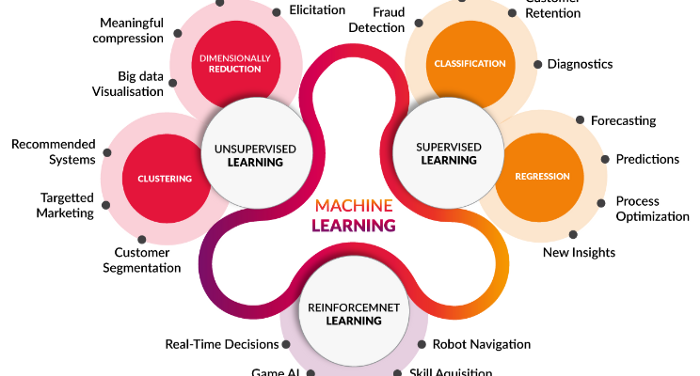
\includegraphics[width=\linewidth]{figures/mlWorld.png}
    \caption{ World of machine learning }
    \source {towardsdatascience.com}
\label{fig:mlWorld}
\end{figure}



%Machine Learning is a term that describes algorithms that learn from data.
%Goodfellow et al. quotes Mitchell from 1996 for a definition of
%what learning means, A computer program is said to learn from experience
%E with respect to some class of tasks T and performance measure P, if its
%performance at tasks in T, as measured by P, improves with experience E.
%There is a wide variety of tasks T that can be done. For instance common
%tasks are regression, classification, anomaly detection, denoising and translation.
%Depending on what experience E they see during the learning process the most
%algorithms can be classified as supervised or unsupervised learning. Supervised
%learning algorithms experience a data set together with target values or labels
%that act as instructions on what to do. The unsupervised learning algorithms
%don’t have any labels or targets but instead try to learn about the structure of
%the data set. The performance P can be how far off from the labels the output
%of the algorithm is in the case of supervised learning. This performance measure
%is often difficult to choose.




Using Machine Learning we can accomplish manly 3 of these following tasks.
\begin{itemize}
\item Regression: Regression attempts to estimate a numerical value from a given number of data points. Forecasting sharemarket or climate, financial audit, for example. There are many types of algorithms for regression analysis. Like – linear, logistic, polynomial, table, [4 in ml], etc.

\item Classification: This technique predicts that a class will be trained on a dataset with many predefined classes. For instance – a model trained on a dataset consists of photos of many animals and then predicts which animal it is when a new image is seen. Multiple types of classification can include binary classifiers, multiclass classifiers. Numerous algorithms are available there for classification. For example – Naive Baias , Decision Trees, and K-Nearest Neighbours. [5 in ml].

\item Clustering: The technology of clustering attempts to identify similarities between data points and to create new clusters with the same data points. When it comes to user behavior research, recommender systems, it is useful to show similarities between data points. For example, a data set consists of data of the customers of a business, using the clustering algorithms on the data set we can group the customer in sections which will help the business to make better decisions. Many well-known clustering algorithms such as – K-means, expectation-maximization, hierarchical, density-based, etc [6 in ml] are available.

\end{itemize}


So we can see there are many forms of machine learning, as we are using Convolutional Neural Network (CNN) withs is a type of Artificial Neural Network, we are going to discuss details about it in the upcoming sections.





\section{Artificial Neural Network}

An Artificial Neural Network usually called neural network is an artificial representation of the human brain. Basically, a neural network is a set of input/output nodes. Each node performs a simple computation by its node function. The connection among the nodes has a weight associated with it. The neural network tries to simulate its learning process.




\begin{figure}[h!]
  \centering
  \begin{subfigure}[b]{0.5\linewidth}
    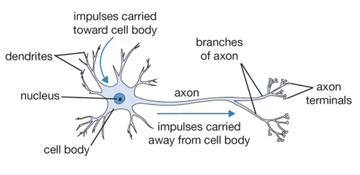
\includegraphics[width=\linewidth]{figures/bgn.png}
    \caption{Single biological neuron}
  \end{subfigure}
\quad
\begin{subfigure}[b]{0.5\linewidth}
    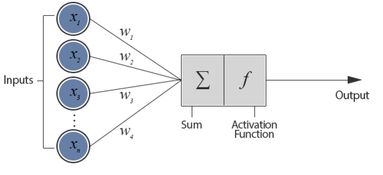
\includegraphics[width=\linewidth]{figures/ann.png}
    \caption{Mathematically modeled biological neuron}
  \end{subfigure}
 \caption{Biological neuron vs artificial neuron}
  \label{fig:bgnVSann}
  \source {datacamp.com}
\end{figure}

An Artificial Neuron tries to mimic the function of neurons in a biological brain. As a biological neuron gets some electric signal from the previous neuron from its dendrite and then passes on the signal if the signal has a certain threshold value through its axon to the next neuron. Together they form millions and billions of connections.
This function of a biological neuron can be mathematically modeled. we get some values and we use an activation function to determine the threshold and can pass it on. The figure represents the functional similarities of a biological and computer-modeled neuron.









\section{Deep Learning}
Deep Learning is a term used for training deep artificial neural networks, or
ANN s. An ANN is a function approximator consisting of multiple functions,

also called neurons. An ANN is called a feedforward ANN if there are no
feedback connections of the output of the ANN being sent to itself. Each neuron
is a linear function of some inputs, fed into a nonlinear function, called activation
function. If the input of a neuron is a vector x, the output of the neuron gi can
be written as


\subsection{Convulitional Neural Network}
The non-linear functions called activation functions, such as K in Equation 2.1,
are typically fixed non-linear functions that are used to make the ANN able to
approximate non-linear functions. If the non-linear activation functions weren’t
used, the output of the ANN would still be a linear function of the inputs x. In deep learning, there are a few commonly used functions that
have become standard as activation functions.
The rectifying linear unit, or ReLU is a function that is defined as


\subsection{Back-propagation}
When training a ANN to approximate a function, gradient based optimization
is commonly used. To compute the gradient of a (loss) function f with
respect to the parameters  an algorithm called back-propagation is commonly
used. It back-propagates from the objective function to gradients of the different
weights and biases in the ANN to compute the gradient of the objective function with respect to all the parameters. If we have a function 
can be a cost function in a supervised learning setting but could also be other
functions like a reward function in the reinforcement learning setting that will

\subsection{Gradient based optimization for deep learning}

The ANN weights and biases are updated to optimize some objective function
with gradient based optimization, using the gradients computed with the backprop algorithm.
The classic algorithm for optimizing the parameters in a ANN is called Gradient
Descent. be an objective function that we want to minimize, where
x is the input to the ANN the trainable parameters of the ANN. Then
moving in the opposite direction of the gradient of L with respect to  we move
the parameters in a direction that makes the objective function smaller, which is
what we want. However, usually x are random samples and the true gradient is
the expected value of the gradient with respect to the random samples actually
used. Thus when computing the gradient of the loss function as a function of
some samples x, we are computing an unbiased noisy estimate of the gradient.
This is referred to as Stochastic Gradient Descent, or SGD. Stochastic Gradient

\subsection{Batch Normalization}
Batch Normalization is a recent method in deep learning used to be able to train
networks faster and use higher learning rates with decreased risk of divergence.
It does so by making the normalization a part of the model architecture, fixing
the mean and variances of the inputs to a layer by a normalization step. This
makes the risk of the inputs to the activation functions getting in a range where
the gradient vanishes smaller and allows for the use of higher learning rates. 

\section{Deep Learning}
Deep Learning is a term used for training deep artificial neural networks, or
ANN s. An ANN is a function approximator consisting of multiple functions,

also called neurons. An ANN is called a feedforward ANN if there are no
feedback connections of the output of the ANN being sent to itself. Each neuron
is a linear function of some inputs, fed into a nonlinear function, called activation
function. If the input of a neuron is a vector x, the output of the neuron gi can
be written as


\subsection{Activation Functions}
The non-linear functions called activation functions, such as K in Equation 2.1,
are typically fixed non-linear functions that are used to make the ANN able to
approximate non-linear functions. If the non-linear activation functions weren’t
used, the output of the ANN would still be a linear function of the inputs x. In deep learning, there are a few commonly used functions that
have become standard as activation functions.
The rectifying linear unit, or ReLU is a function that is defined as

\subsection{Cost Functions}
To train a ANN, cost functions are usually minimized. In supervised learning, where we have labeled data to learn from, the cost functions are more
straightforward than for instance in reinforcement learning that we will discuss
in section 
The two main problems of supervised learning are regression and classification.
In regression one wants to predict a numerical value whereas in classification the
goal is to predict which class something belongs to given some inputs. Different
loss functions are common for regression and classification. Most of them are
however derived from the same principle, the one of Maximum Likelihood.

\subsection{Back-propagation}
When training a ANN to approximate a function, gradient based optimization
is commonly used. To compute the gradient of a (loss) function f with
respect to the parameters  an algorithm called back-propagation is commonly
used. It back-propagates from the objective function to gradients of the different
weights and biases in the ANN to compute the gradient of the objective function with respect to all the parameters. If we have a function 
can be a cost function in a supervised learning setting but could also be other
functions like a reward function in the reinforcement learning setting that will

\subsection{Gradient based optimization for deep learning}

The ANN weights and biases are updated to optimize some objective function
with gradient based optimization, using the gradients computed with the backprop algorithm.
The classic algorithm for optimizing the parameters in a ANN is called Gradient
Descent. be an objective function that we want to minimize, where
x is the input to the ANN the trainable parameters of the ANN. Then
moving in the opposite direction of the gradient of L with respect to  we move
the parameters in a direction that makes the objective function smaller, which is
what we want. However, usually x are random samples and the true gradient is
the expected value of the gradient with respect to the random samples actually
used. Thus when computing the gradient of the loss function as a function of
some samples x, we are computing an unbiased noisy estimate of the gradient.
This is referred to as Stochastic Gradient Descent, or SGD. Stochastic Gradient



% !TeX root = ../main.tex
% Add the above to each chapter to make compiling the PDF easier in some editors.

\chapter{Relatedwork}\label{chapter:relatedwork}


% !TeX root = ../main.tex
% Add the above to each chapter to make compiling the PDF easier in some editors.

\chapter{Simulation Setup}\label{chapter:simulation_setup}
The Experiment Setup can be divided into two phases, one is set up the simulation and collect data from the simulated setup. We call title this two-section as Simulation and Data Collection respectively.
In this section we describe the detailed information for the simulation software and how we gathered data from the simulation and preprocessed the data to feed in the CNN algorithm.

We use simulated data because its easier to deal without any noise and doesn't need calibration and registration. The other advantages of the simulated data are that the simulated environment is ideal for this kind of experiment without any noisy data and its ideal for the analysis of the result before using it into the real world scenario and compare with it.

We obtained the from the simulation as .txt formate. then we processed the data and convert the data points in csv formate to use in our CNN model.

\section{Simulation}
As for the simulation we need to choose a simulation software that fulfills our requirement for simulating IMUs and moving the sensors on a flat plane on a predefined path. The other crucial requirements were, the data must be faultless and noise-free. For example, the item that had been utilized to mount the IMUs needed to move openly satisfying Six Degrees of Freedom (6DoF). 

Moreover, the estimations from the virtual IMUs must be as exact as conceivable to imitate a real situation. We had fewer options for the simulation software to choose from. Among the simulation software we checked for our simulation MATLAB and CoppeliaSim Robotics were better performing.

\subsection{Simulation software}
After intensive investigation, we chose to go with the CoppeliaSim Robotics Education version for our simulation tool. Beforehand this product was known as V-Rep by Coppelia Robotics. One of the primary purposes behind picking this simulation tool is the assortment of accessible simple to utilize alternatives to mimic genuine situations. This product is created to recreate genuine situations for various mechanical parts for example Robot arms, Hexapods. It additionally has a wide scope of different segments for reproduction purposes. For instance – Infrastructure, furniture, family unit things, office things, and even people for reenactment purposes. This product offers a scope of usable virtual sensors for example – accelerometers, spinners, vision sensors, laser scanner, GPS sensors, and so forth. 

The training adaptation is free for all. Since we didn't need to stress over the frequencies of various IMUs since every one of them is reproduced, the CPU recurrence made a difference the most while gathering the information. To analyze the reason, we ran the recreation on various CPU load. For example, with 4 IMUs and no other application running on the foundation, it took roughly 73 minutes to gather 1,06,437 information focuses. In a similar arrangement, however, with Google Chrome running on the foundation, the reenactment could just gather 47,509 information focuses on a similar time. It is required to run the reproduction remain solitary to get around the comparative number of information that focuses on a comparable time period.

In the following section we will describe the the components of the CoppeliaSim Robotics and how we used it to create the simulation 

\subsection{Scene Object}


\begin{figure}[h!]
  \centering
  \begin{subfigure}[b]{0.4\linewidth}
    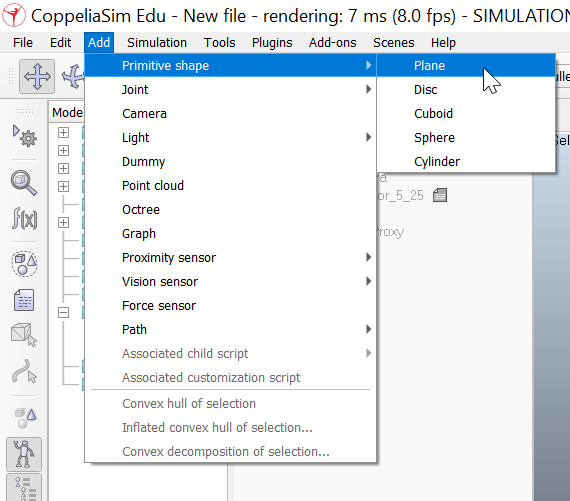
\includegraphics[width=\linewidth]{figures/adding_2d_plane.png}
    \caption{2D plane to the scene.}
  \end{subfigure}
  \begin{subfigure}[b]{0.4\linewidth}
    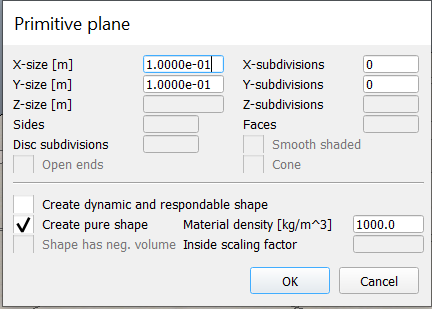
\includegraphics[width=\linewidth]{figures/config_plane.png}
    \caption{Plane Configaration.}
  \end{subfigure}
 \begin{subfigure}[b]{0.6\linewidth}
    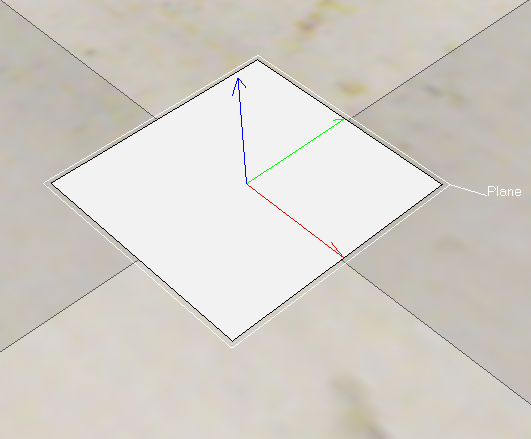
\includegraphics[width=\linewidth]{figures/plane.png}
    \caption{Created 2D plane.}
  \end{subfigure}
  \caption{Creating scene object.}
  \label{fig:scene_object}
\end{figure}

To recreate a real-world like situation, the main thing we required was an object for the scene. The object would represent the qualities of a moving segment in the simulated scenario

For our investigation, we required an object to contain the IMUs that would move along on a pre-characterized way. Obviously, 6 DoF must be guaranteed to make however much as could reasonably be expected accurate data. For our first methodology, we utilized effectively accessible predefined shapes that built-in the software. The software gives a number of predefined shapes such as plane, circle, cuboid, circle, and cylinder. We picked to utilize a two-dimensional plane as our object since it is the nearest to our model scenario. 



The plane is sufficiently large to contain at least 16 IMUs which is the most noteworthy number of IMUs we chose to utilize. The examples for putting the IMUs on the plane had been chosen together which would in the end help us to get the most ideal and solid information. 

To add our ideal object to the scene, the following steps were :
\begin{enumerate}
  \item Click on ‘Add’ on the menu bar.
  \item Go to the first option; ‘Primitive Shape’.
  \item Click on ‘Plane’ to add a two dimensional plane in our scene.
  \item No change needed in the ‘Primitive plane’ dialog box and click ‘OK’.
\end{enumerate}


\section{Inertial Measurement Units}

The next task is to add IMUs (Inertial Measurement Units) into our plane. The IMU containes an accelerometer and a gyroscope sensor. In the sensor section of the simulation tool, there is no IMU sensor out of the box but there are an accelerometer and a gyroscope sensor. To create IMU we combined these 2 sensors and added to to our plane. 

To add one of those sensors to our scene, the following steps are needed to be followed:

\begin{enumerate}
  \item Click on ‘components’ on the ‘Model browser’ pane.
  \item Click on ‘sensors’; this would open a new pane for all the available sensors just below the browser pane.
  \item Scroll down the pane to select our desired sensors (accelerometer, gyroscope).
  \item Drag and drop the sensors on our plane in the scene.
\end{enumerate}


\begin{figure}[h!]
    \centering
    \setkeys{Gin}{height=45mm}
        \subfloat[selection sensor componant.]{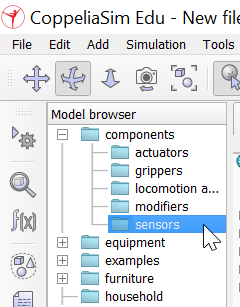
\includegraphics{figures/selecting_sensor_componant.png}}
        \quad
        \subfloat[selction accelerometer and a gyroscope sensor.]{%
            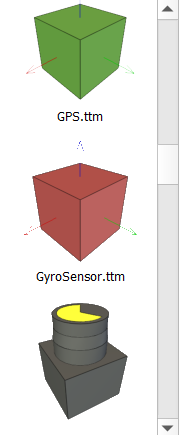
\includegraphics{figures/selecting_gyro_acc_componant.png}}
        \caption{Creating IMU.}
        \label{fig:creating_IMU}
    \end{figure}

To combine the accelerometer and a gyroscope sensor and make a single IMU we need to change the LUA script attached with every sensor. Although it was possible just to drag and drop the sensors but we wanted to create a custom script to add a single unit IMU to incorporate our custom simulation control panel. we will discuss the control panel later on in the upcoming section. 

\subsection{Making IMU}

We created a custom IMU combining gyroscope and accelerometer in a separate scene. To do that we selected the gyrosensor script as our base script. Then we added the accelerometer into the scene with the gyrosensor. Both of the components Lua scripts were auto-generated which can sense and collect data by the software. We changed the Lua script for both of the gyrosensor and accelerometer to get the sensor data out of the software and saved in a .txt file. When we are satisfied with our work, we saved the whole script as a new sensor names IMU. This IMU now consists of one accelerometer and one gyroscope also we can add 1  to 16 number of IMU from our custom control panel.

\begin{figure}[h]
  \centering
    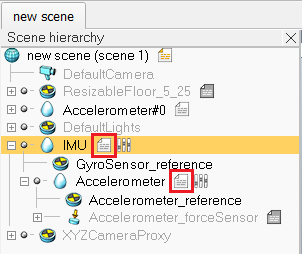
\includegraphics[width=8cm]{figures/IMU_Creation.png}
    \caption{IMU Creation.}
\end{figure}

It is important to mention, the autogenerated script was in the non-threaded mode, if we write in nonthreaded mode all the data gets overwritten by the last sensor data. we hade to wrote threaded scripts get out of this situation.

\subsection{IMU pattern in a 2D plane}

In sensor fusion, the number of IMU and the position of IMU plays a very important role. For that, it was very important for was to experiment with what number of IMU in which position gives us the best result. One of our primary objectives was to try the combination of IMU (2 to 16) in the simulation. 
It was very important to try different experiments with this number of IMUs for this particular issue scope. 
[..] have explored different avenues regarding 8 real IMUs joined on a circuit board to gather real-world information, yet not utilizing various examples with various numbers of IMUs. It is a direct result of the very complex nature of the task to connect and segregate IMUs after each and every run. At that point comes the issue of calibration; which is meticulous in light of the fact that each time another IMU is joined or an IMU gets disengaged all the rest of the IMUs should be adjusted one by one.

Using a simulation instead of a real-world sensor comes handy in this type of situation. Just using a mouse click we can change the number of IMU from our custom control panel without needing any calibration or registration. To identify the patterns of IMU we need a bit of trial and testing since we didn't have any benchmark for IMU designs. We took []'s work with 8 IMUs as our base and characterized the examples for the IMUs around it. Moreover, we thought about the alignment and situating for various IMUs for a genuine gadget, which in the long run helped us to settle the examples. 

The accompanying figures give a diagram of the pattern designs for the IMUs:

\begin{figure}[h!]
  \centering
  \begin{subfigure}[b]{0.2\linewidth}
    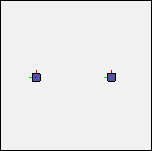
\includegraphics[width=\linewidth]{figures/IMU2.png}
    \caption{2 IMU pattern }
  \end{subfigure}
\begin{subfigure}[b]{0.2\linewidth}
    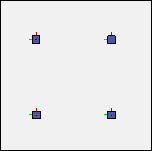
\includegraphics[width=\linewidth]{figures/IMU4.png}
    \caption{4 IMU pattern.}
  \end{subfigure}
\begin{subfigure}[b]{0.2\linewidth}
    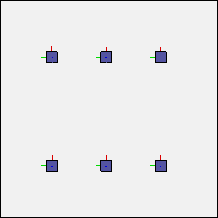
\includegraphics[width=\linewidth]{figures/IMU6.png}
    \caption{6 IMU pattern.}
  \end{subfigure}
\begin{subfigure}[b]{0.2\linewidth}
    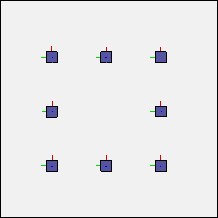
\includegraphics[width=\linewidth]{figures/IMU8.png}
    \caption{8 IMU pattern.}
  \end{subfigure}

 \begin{subfigure}[b]{0.2\linewidth}
    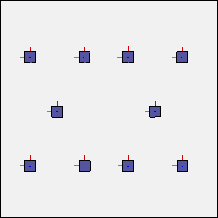
\includegraphics[width=\linewidth]{figures/IMU10.png}
    \caption{10 IMU pattern.}
  \end{subfigure}
  \begin{subfigure}[b]{0.2\linewidth}
    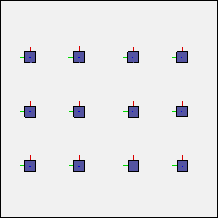
\includegraphics[width=\linewidth]{figures/IMU12.png}
    \caption{12 IMU pattern.}
  \end{subfigure}
  \begin{subfigure}[b]{0.2\linewidth}
    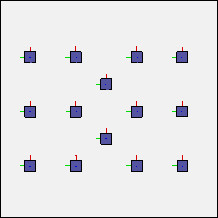
\includegraphics[width=\linewidth]{figures/IMU14.png}
    \caption{14 IMU pattern.}
  \end{subfigure}
  \begin{subfigure}[b]{0.2\linewidth}
    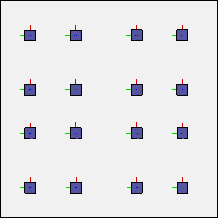
\includegraphics[width=\linewidth]{figures/IMU16.png}
    \caption{16 IMU pattern}
  \end{subfigure}

  \caption{Number of IMU position on a 2D plane.}
  \label{fig:IMU_pattern}
\end{figure}



Although we initially try to test every pattern from 1 to 16 but we end up using an even number of IMUs for our purpose to reduce the time for CNN testing and there was no significant difference from changing 2 IMU to 3 IMU then 4 IMU. 


\section{Simulation Path}

As we are prediction position and orientation of an object, we need a path in our simulation where our dummy object will go through. Therefore creating a simulated path as close as possible to real trajectory was one of the main concerns. Our path has to be in such a way where our object can move with 6Dof. In our simulation tool the path controllers the position and orientation of the moving object in our case the 2D plane. We need to create the paths with multiple rotation and elevation where our object will move and we can collect the data of the position and orientation, in short, the pose of the object.

\begin{figure}[h]
  \centering
    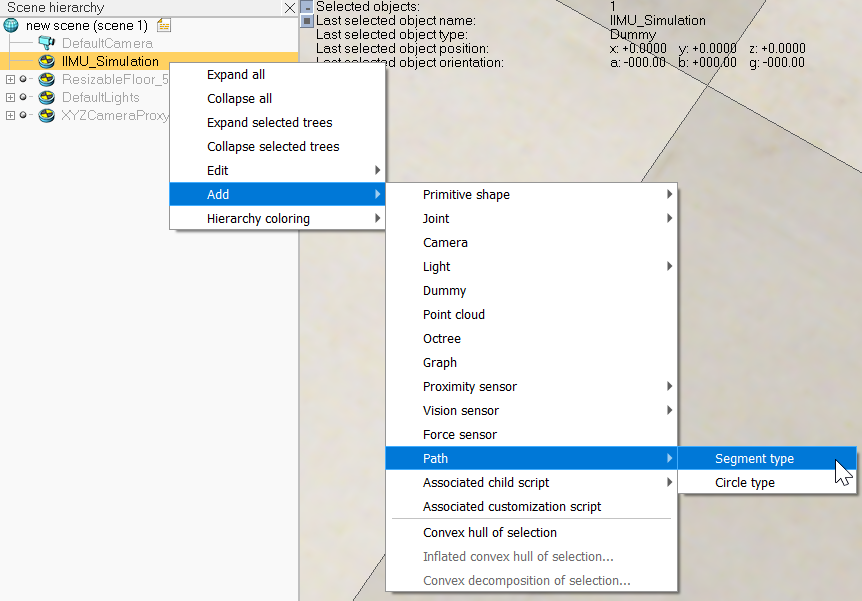
\includegraphics[width=\linewidth]{figures/pathCreation.png}
    \caption{Path Creation.}
\label{fig:Path_creation}
\end{figure}


We need a large amount of dataset to train our Neural Network for that our path has to be long enough with orientation, with elevation gain and loss to generate the data. Meaning our plane with the IMU and dummy object will go up and down, left and right rotation along the path. These features need to ensure by the path design itself. The path design also facilitates other features slike roll, pitch, and yaw. 

\subsection{Dummy Object}
To control our simulation environment we need a control panel, to do that we need an entry point. The creation of a dummy object makes the process easier. we need to add our customize script to the dummy object script to make our control panel. that's why adding a dummy object is very important. The detail about the control panel will be discussed in the upcoming section.
We can simply add a dummy object from the simulation tool using the following steps: 

\begin{enumerate}
  \item  Navigate to the ‘Scene hierarchy’ pane.
  \item  Right click on the scene name.
  \item Go to ‘Add’ and click on ‘Dummy’
\end{enumerate}



\begin{figure}[h!]
  \centering
  \begin{subfigure}[b]{0.4\linewidth}
    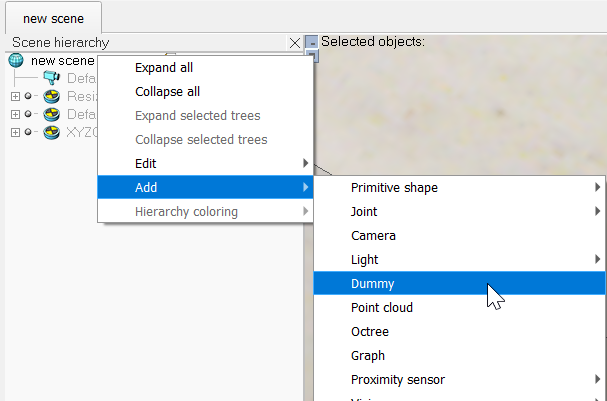
\includegraphics[width=\linewidth]{figures/addingDummyObject.png}
    \caption{Adding Dummy Object }
  \end{subfigure}
\quad
\begin{subfigure}[b]{0.4\linewidth}
    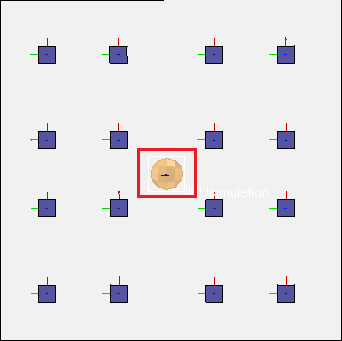
\includegraphics[width=\linewidth]{figures/DummyObjectinaPlane.png}
    \caption{Dummy Object in a Plane.}
  \end{subfigure}
 \caption{Dummy Object.}
  \label{fig:Dummy_object}
\end{figure}

After creating the dummy object we named it IMU Simulation  and we placed it in the center  (x, y, z : 0, 0, 0)  of the plane.


\subsection{Creating the path for the plane}

The path creation process was really time-consuming. In the beginning, we started just adding a default path from the simulation tool. There are 2 types of paths in the tool one is circular path another is the segmented path. As we needed path with many orientation and elevation we selected the segmented path showed in figure ~\ref{fig:Path_creation}.
The following steps are taken to add a segmented path in the scene:

\begin{enumerate}
  \item Go to the ‘Scene hierarchy’ pane.
  \item Right-click on IMU Simulation.
  \item Go to ‘Add’ and then go to ‘Path’.
  \item Click on ‘Segment type’ to create the primitive path.
\end{enumerate}

The segmented path just adds a straight line in the scene. At first, we added many segmented paths in the scene but when we tried to join them together it was cumbersome.
Then we decided to modify a single segmented path by adding many path control points and give it random elevation, orientation, and trajectory. To do that we need to go to the section called Path edit mode.

\subsubsection{Path Control Points}


In order to manipulate our segmented path we took a single segmented path and created many path points. Adding path points is fairly easy on the simulation tool.
Select the path from the scene.

\begin{figure}[h!]
  \centering
  \begin{subfigure}[b]{0.5\linewidth}
    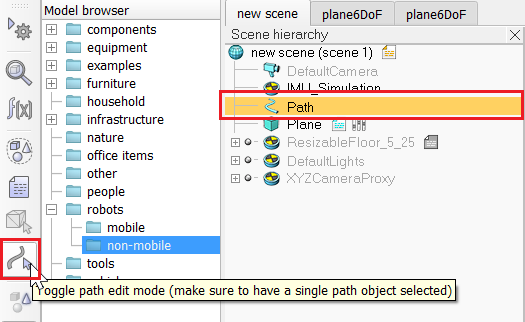
\includegraphics[width=\linewidth]{figures/PathControllPoint.png}
    \caption{Adding Path Control Points}
  \end{subfigure}
\quad
\begin{subfigure}[b]{0.5\linewidth}
    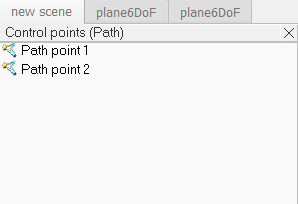
\includegraphics[width=\linewidth]{figures/PathControllPointsPane.png}
    \caption{After Path Controll Points are added.}
  \end{subfigure}
 \caption{Path Control Points.}
  \label{fig:PathControlPoint}
\end{figure}

\begin{enumerate}
  \item Click the path edit mode shown in the figure ~\ref{fig:PathControlPoint}
  \item Go to the control point section and right-click on it.
  \item From the menu, select Insert new control point after selection.
\end{enumerate}

We repeated these steps many times to make our path longer as we needed. 

The new point gets made right on the last point, or essentially put the point we chose to include the new point. To move the recently included point, from the outset we have to choose the point and afterward switch 'Object/Item shift' button on the top control panel. After we selected a control point in the scene, we just drag and drop in our desired position. This choice permits moving any article in the scene along with all the three-axis. Two kinds of movement are permitted through this process:

\begin{enumerate}
  \item Move an object along the X-axes and Y-axes by using the mouse; by simple drag and drop.
  \item Right-click on IMU Simulation.
  \item Press ‘CTL’ in the keyboard and moving the cursor up and down to move the object along Z-axis.
\end{enumerate}

We had to do these steps for every control points over our whole path.


\subsubsection{Path Orientation}

After we created the long path we run the simulation. The simulation was running well and we collected 20 minutes of simulation data. When we were analyzing the data we found that the object orientating in one axis. As we need 6Dof we can not take the data from the simulation. 

After investigating we found to change the orientation of our plane we need to change in the path control points. But, the method or the ability to add a configuration script to adjust the path Control points orientation is not available automatically from the tool. We need to change every control point we added in our simulation path. This was a time-consuming process. The longer the path the more control point we had to change. After a considerable amount of time, we change the control points and run the simulation again. This time our plane was oriented along the 3 axes but there was a problem. The object was only changing its orientation only at the control point but not along the path. For better explanation lets say, The plane was moving from control point A to control point B then to control point C. The plane is only changing its orientation axis when it reaches the control point B and keeps its orientation along the path From B to C and then change its orientation again in point C. This is not what we wanted.

We tried to solve this problem by turning on the "Automatic Orientation" checkbox in the path edit mode dialog box for orientation. By default, this box was checked. With this activated option, the object that moves along the path should frequently change its angles. But in simulation, it does not. The object only keeps the roll but not yaw and pitch. The characteristics of 6 
DoF are thus violated.

\begin{figure}[h]
  \centering
    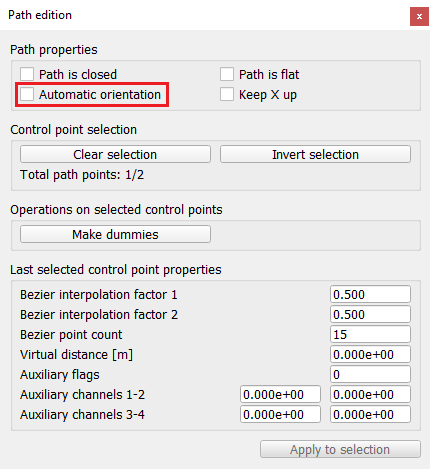
\includegraphics[width=0.4\linewidth]{figures/uncheckAuto.png}
    \caption{Toggle Autometic Rotation.}
\label{fig:TAutoRotation}
\end{figure}

After a lot of investigation, the only solution we came up with is to add a lot more control points with a variant of angle values.  To do that first we need to check out the ‘Automatic Orientation’ option from the Path edit panel. This enables us to move the object in our case the 2D pane with 6DoF.
Creating control points with the very near proximity of multiple angles frequently, resembles the actual close to a real-world scenario. One thing that should be remembered here is that this configuration doesn't remove our missing Pitch, Yaw problem.


\begin{figure}[h!]
  \centering
  \begin{subfigure}[b]{0.4\linewidth}
    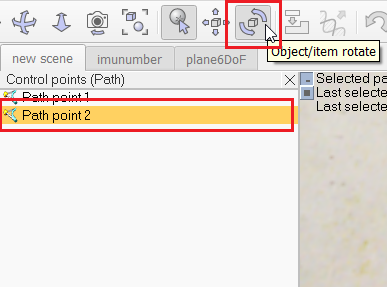
\includegraphics[width=\linewidth]{figures/toggleRotation.png}
    \caption{Rotating the control point}
  \end{subfigure}
\quad
\begin{subfigure}[b]{0.4\linewidth}
    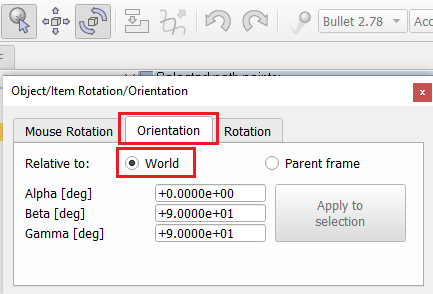
\includegraphics[width=\linewidth]{figures/changingAngles.png}
    \caption{Changing the Angles .}
  \end{subfigure}
 \caption{Orientation of control points.}
  \label{fig:orientationControlPoints}
\end{figure}


The following steps are necessary to set the orientation values by changing the control points' default angle values: 

\begin{enumerate}
 \item	Select the latest point on the ‘Control points’ pane.
 \item.	Click the ‘Object/Item’ rotate on the top control pane. Doing this opens a new control panel for orientation and rotation for that particular control point.
 \item	Navigate to the ‘Orientation’ tab.
 \item	Make sure orientation is relative to the world frame.
 \item.	Change the angle values (alpha, beta, and gamma) and click ‘Apply to selection’.
\end{enumerate}

After we fix all the contorl panel our path look like the followinge figure.

\begin{figure}[h]
  \centering
    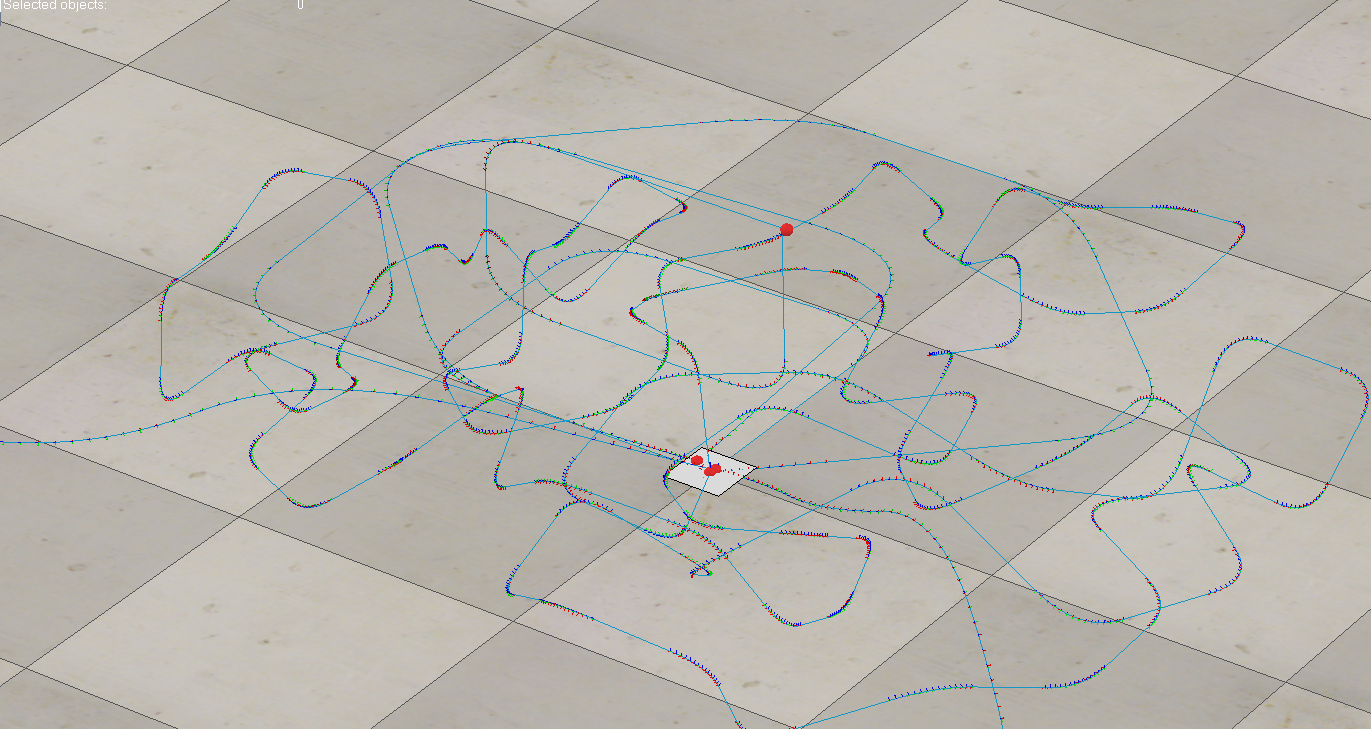
\includegraphics[width=0.9\linewidth]{figures/finalPath.png}
    \caption{Final simulation path.}
\label{fig:finalPath}
\end{figure}

In the next section we will describe how we created a customize control panel for the simulation.


\section{Customized Control Panel}

We want to have a control panel to run our simulation. We could run to simulation from the 'CoppeliaSim' tool itself but we wanted to have some graphical user interface (GUI) to control our simulation. The customize GUI allows us to easily change the simulation environment such as Number of IMU, Object Velocity, Object Acceleration, and the Path should follow. Otherwise, we had to change the simulation script every time we run the simulation.

\begin{figure}[h]
  \centering
    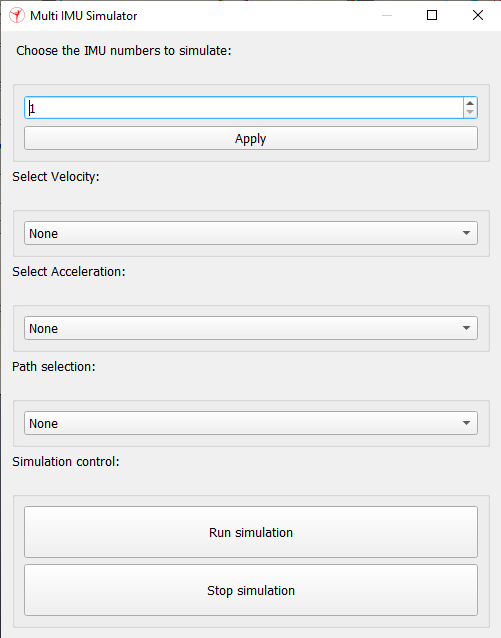
\includegraphics[width=0.6\linewidth]{figures/simCPanel.png}
    \caption{Simulation control panel.}
\label{fig:simCP}
\end{figure}


Our control panel GUI was fairly simple and user friendly. We highlighted the 'Run simulation' and 'Stop simulation' button bigger to access easily because these are the buttons we used most. 
The other options were:
\begin{enumerate}
  \item Number of IMU: this is a drop-down menu where we can easily select how many numbers of IMUs should be on the plane. The range is from 1 to 16 with predefined positions.
  \item Select Velocity: We had three predefined velocity option in this drop-down menu. The predefined options are 0.01, 0.03, 0.05 meter per second.
  \item Select Acceleration: As like the 'Select velocity'  menu we predefined the acceleration parameter in the dropdown menu.
  \item Path selection: As we tested our simulation in multiple paths. In this dropdown section, we put the name of the path to select to run the simulation in that path. From the beginning, we created 6 different paths so we named them accordingly. Such as Path1, Path2 till Path6 
\end{enumerate}


\subsection{Creating the options for the control panel}

The GUI of the control panel created using simple XML. All the options from the GUI to work we need to add customized Lua Script in our simulation tool. As the starting point of our simulation is our Dummy Object, we had to add the customize Lua Script in the script of the Dummy object.

\begin{figure}[h]
  \centering
    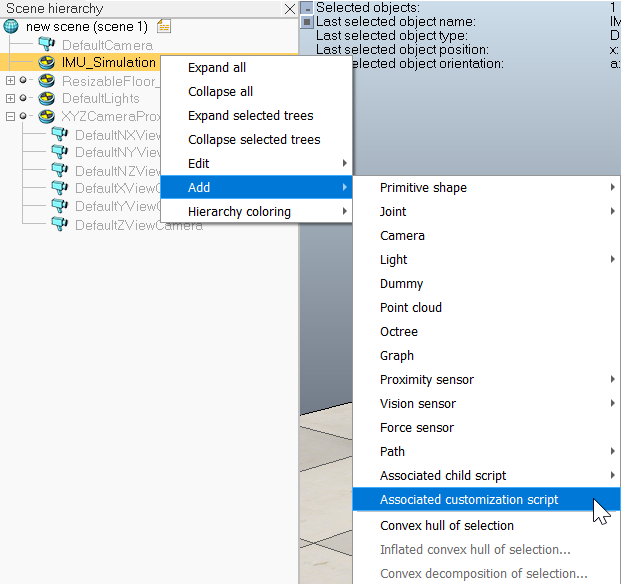
\includegraphics[width=0.6\linewidth]{figures/assoChildScript.png}
    \caption{Customizing the script to create the control panel.}
\label{fig:assoCS}
\end{figure}

We added the necessary methods such as the functions for velocity and acceleration in this associated child script of the Dummy Object.


\section{Data Collection} \label{dataCollection}
Collection of the Data for training our Neural Network model consists of two parts. One is collecting the data of the sensors(IMU) which will be our input data for the model and the other is collecting the data from the dummy object which we call the ground truth will be out label data for our model.
Primarily we collected data both for ground truth and the IMU data out of the simulation as a txt file. The formate of the data will be discussed in the section: "" . Then we Fromate the data as per our requirement for the Neural Network Model.

It is important to note that, We spent a lot of time preprocessing the data to feed our model. The primary data set will be changed into as a csv formate after we preprocess the data as we need csv formate to feed our model in google collab []. We will discuss preprocessing in the Experiment setup [] section. It is very important to know about the shape of our data to know and identify how our data is going through the network. That is why we took every sensor data in different file formate. Without knowing the shape and size of the data without it, data processing and feeding into the neural networks are incredibly difficult.

\subsection{Sensor (IMU) Data}
We collected each of the Sensor data in different .txt file. The number of the data file, in this case, depending on the number of IMU we have in our simulation. For example, if we have 4 IMU in our simulation we have 8 data files. 2 files for each IMU, one is for the gyroscope data and the other for the accelerometer data. We could have collected the data in a single file but we decided to separate the initial data because it will help us to preprocess the data for better reliability and manipulation. The data formate for the sensor data is given below.

Data formate for the accelarometer :
\begin{table}[h]
\begin{tabular}{lllll}
 timestamp\_1 & a\_x &  a\_y &  a\_z  \\
 timestamp\_2 & a\_x &  a\_y &  a\_z   \\
…. & …. &  …. & ….  \\
…. & …. &  …. & ….  \\
 timestamp\_n & a\_x &  a\_y &  a\_z 
\end{tabular}
\end{table}



Data formate for the gyroscope:

\begin{table}[h]
\begin{tabular}{lllll}
 timestamp\_1 & $ \omega $ \_x &   $ \omega $\_y &   $ \omega $\_z  \\
 timestamp\_2 & $ \omega $ \_x &   $ \omega $\_y &   $ \omega $\_z  \\
…. & …. &  …. & ….  \\
…. & …. &  …. & ….  \\
 timestamp\_n & $ \omega $ \_x &   $ \omega $\_y &   $ \omega $\_z 
\end{tabular}
\end{table}



The explanation for calling columns a\_x, a\_y, and a\_z of the accelerometer is that 'a' is the unit of acceleration and is readable easily. The same applies to the columns of gyroscopic data "$ \omega $" as the angular velocity unit.

\subsection{Ground Truth}

As we said before the ground truth data is the label for the training of our model. The word 'ground truth' in machine learning refers to the precision of the evaluation of learning methods by the training sets. It is used to support or deny scientific theories in mathematical models.  In terms of our goal, the ground truth is the precise position and orientation (pose) of the object in a particular timestamp. We took milliseconds difference from each timestamp.

In our training data set, the input data will be feed into the model and try to mimic the result as close as possible with the ground truth. Ground truth values are extremely crucial to the validation process. So we have to be very careful to have the precise ground truth values from the dummy object in our simulation.
Another important point to note, The number of ground truth readings should be equal to the number of IMU reading, this way we tried to somewhat synchronize the IMU and ground-truth data. The explanation behind this is that "NaN" values should not be obtained by using a test path dataset to determine the efficiency of one of our trained models.

Normally we should get the ground truth data from the script written in the dummy object attached to the plane but we faced problems with the ground truth values of the script attached to the plane. 
For unexplained reasons, several values were absent. The CPU was not able to sense the IMU sub-script, which is the accelerometer script, as we thought. 
We carried out further experiments to integrate the ground truth script into the IMU. After several tests, the ground truth value was finally obtained by using the script in the associated Gyroscope script with similar data point counts. We used the gyroscope script as the parent IMU script.

Data formate for the Ground Truth:

\begin{table}[h]
\begin{tabular}{lllllll}
 timestamp\_1 &  t\_x &   t\_y &   t\_z &   o\_x &   o\_y  &  o\_z \\
  timestamp\_2 &  t\_x &   t\_y &   t\_z &   o\_x &   o\_y  &  o\_z \\
…. & …. &  …. & …. & …. & …. & …. \\
…. & …. &  …. & …. & …. & …. & ….  \\
 timestamp\_n &  t\_x &   t\_y &   t\_z &   o\_x &   o\_y  &  o\_z
\end{tabular}
\end{table}


We have 1 data file for the ground truth for each simulation run. The file contains seven data columns. The 1st one is the timestamp in milliseconds, the next three are the position coordinates of the plane across three axes and the last three columns contain the plane’s orientation across three axes in degrees. Seven data points in each row make the pose of the plane. It is important to note the orientation calculated in relation to the "World frame" which is the whole simulation frame. 


%\begin{figure}[h!]
%  \centering
%  \begin{subfigure}[b]{0.4\linewidth}
%    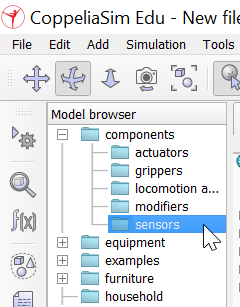
\includegraphics[width=\linewidth]{figures/selecting_sensor_componant.png}
%    \caption{Coffee.}
%  \end{subfigure}
%  \begin{subfigure}[b]{0.4\linewidth}
%    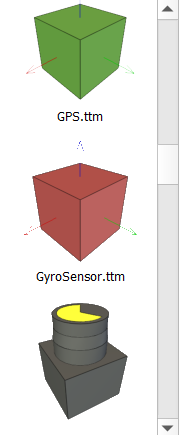
\includegraphics[width=\linewidth]{figures/selecting_gyro_acc_componant.png}
%    \caption{More coffee.}
%  \end{subfigure}
%  \caption{The same cup of coffee. Two times.}
%  \label{fig:coffee}
%\end{figure}


% !TeX root = ../main.tex
% Add the above to each chapter to make compiling the PDF easier in some editors.

\chapter{Experiment Setup}\label{chapter:experiment_setup}
The Experiment Setup can be divided into two phases, one is set up the simulation and collect data from the simulated setup. We call title this two-section as Simulation and Data Collection respectively.
In this section we describe the detailed information for the simulation software and how we gathered data from the simulation and preprocessed the data to feed in the CNN algorithm.
We use simulated data because its easier to deal without any noise and doesn't need calibration and registration. The other advantages of the simulated data are that the simulated environment is ideal for this kind of experiment without any noisy data and its ideal for the analysis of the result before using it into the real world scenario and compare with it.

We obtained the from the simulation as .txt formate. then we processed the data and convert the data points in csv formate to use in our CNN model.

\section{Simulation}
As for the simulation we need to choose a simulation software that fulfills our requirement for simulating IMUs and moving the sensors on a flat plane on a predefined path. The other crucial requirements were, the data must be faultless and noise-free. For example, the item that had been utilized to mount the IMUs needed to move openly satisfying Six Degrees of Freedom (6DoF). Moreover, the estimations from the virtual IMUs must be as exact as conceivable to imitate a real situation. We had fewer options for the simulation software to choose from. Among the simulation software we checked for our simulation MATLAB and CoppeliaSim Robotics were better performing.

\subsection{Simulation software}
After intensive investigation, we chose to go with the CoppeliaSim Robotics Education version for our simulation tool. Beforehand this product was known as V-Rep by Coppelia Robotics. One of the primary purposes behind picking this simulation tool is the assortment of accessible simple to utilize alternatives to mimic genuine situations. This product is created to recreate genuine situations for various mechanical parts for example Robot arms, Hexapods. It additionally has a wide scope of different segments for reproduction purposes. For instance – Infrastructure, furniture, family unit things, office things, and even people for reenactment purposes. This product offers a scope of usable virtual sensors for example – accelerometers, spinners, vision sensors, laser scanner, GPS sensors, and so forth. The training adaptation is free for all. Since we didn't need to stress over the frequencies of various IMUs since every one of them is reproduced, the CPU recurrence made a difference the most while gathering the information. The CPU must be liberated from use from different applications while the information assortment process is going on. To analyze the reason, we ran the recreation on various CPU load. For example, with 4 IMUs and no other application running on the foundation, it took roughly 73 minutes to gather 1,06,437 information focuses. In a similar arrangement, however, with Google Chrome running on the foundation, the reenactment could just gather 47,509 information focuses on a similar time. It is required to run the reproduction remain solitary to get around the comparative number of information that focuses on a comparable time period.

% !TeX root = ../main.tex
% Add the above to each chapter to make compiling the PDF easier in some editors.

\chapter{Experiment setup and Methodology}\label{chapter:experiment_setup}
In this chapter we will discuss about our experiment setup and methodology for training our neural network models. Our goal is to preprocess the data from our simulation software in a format that we can feed it to the neural network models, then train the models. The data we got from our simulation is not suitable for direct feeding to the neural network because different models have different structure for the input of the data. We will also discuss the mythology behind the formatting of the data and our experiment setup and also the architectures of our Convolutional Neural Network (CNN).


\section{Data Pre-Processing}

















































Citation test~\parencite{latex}.

\subsection{Subsection}

See~\autoref{tab:sample}, \autoref{fig:sample-drawing}, \autoref{fig:sample-plot}, \autoref{fig:sample-listing}.

\begin{table}[htpb]
  \caption[Example table]{An example for a simple table.}\label{tab:sample}
  \centering
  \begin{tabular}{l l l l}
    \toprule
      A & B & C & D \\
    \midrule
      1 & 2 & 1 & 2 \\
      2 & 3 & 2 & 3 \\
    \bottomrule
  \end{tabular}
\end{table}

\begin{figure}[htpb]
  \centering
  % This should probably go into a file in figures/
  \begin{tikzpicture}[node distance=3cm]
    \node (R0) {$R_1$};
    \node (R1) [right of=R0] {$R_2$};
    \node (R2) [below of=R1] {$R_4$};
    \node (R3) [below of=R0] {$R_3$};
    \node (R4) [right of=R1] {$R_5$};

    \path[every node]
      (R0) edge (R1)
      (R0) edge (R3)
      (R3) edge (R2)
      (R2) edge (R1)
      (R1) edge (R4);
  \end{tikzpicture}
  \caption[Example drawing]{An example for a simple drawing.}\label{fig:sample-drawing}
\end{figure}

\begin{figure}[htpb]
  \centering

  \pgfplotstableset{col sep=&, row sep=\\}
  % This should probably go into a file in data/
  \pgfplotstableread{
    a & b    \\
    1 & 1000 \\
    2 & 1500 \\
    3 & 1600 \\
  }\exampleA
  \pgfplotstableread{
    a & b    \\
    1 & 1200 \\
    2 & 800 \\
    3 & 1400 \\
  }\exampleB
  % This should probably go into a file in figures/
  \begin{tikzpicture}
    \begin{axis}[
        ymin=0,
        legend style={legend pos=south east},
        grid,
        thick,
        ylabel=Y,
        xlabel=X
      ]
      \addplot table[x=a, y=b]{\exampleA};
      \addlegendentry{Example A};
      \addplot table[x=a, y=b]{\exampleB};
      \addlegendentry{Example B};
    \end{axis}
  \end{tikzpicture}
  \caption[Example plot]{An example for a simple plot.}\label{fig:sample-plot}
\end{figure}

\begin{figure}[htpb]
  \centering
  \begin{tabular}{c}
  \begin{lstlisting}[language=SQL]
    SELECT * FROM tbl WHERE tbl.str = "str"
  \end{lstlisting}
  \end{tabular}
  \caption[Example listing]{An example for a source code listing.}\label{fig:sample-listing}
\end{figure}

% !TeX root = ../main.tex
% Add the above to each chapter to make compiling the PDF easier in some editors.

\chapter{Experiment Results and Comparison}\label{chapter:experiment_results_and_comparison}

\section{Section}
Citation test~\parencite{latex}.

\subsection{Subsection}

See~\autoref{tab:sample}, \autoref{fig:sample-drawing}, \autoref{fig:sample-plot}, \autoref{fig:sample-listing}.

\begin{table}[htpb]
  \caption[Example table]{An example for a simple table.}\label{tab:sample}
  \centering
  \begin{tabular}{l l l l}
    \toprule
      A & B & C & D \\
    \midrule
      1 & 2 & 1 & 2 \\
      2 & 3 & 2 & 3 \\
    \bottomrule
  \end{tabular}
\end{table}

\begin{figure}[htpb]
  \centering
  % This should probably go into a file in figures/
  \begin{tikzpicture}[node distance=3cm]
    \node (R0) {$R_1$};
    \node (R1) [right of=R0] {$R_2$};
    \node (R2) [below of=R1] {$R_4$};
    \node (R3) [below of=R0] {$R_3$};
    \node (R4) [right of=R1] {$R_5$};

    \path[every node]
      (R0) edge (R1)
      (R0) edge (R3)
      (R3) edge (R2)
      (R2) edge (R1)
      (R1) edge (R4);
  \end{tikzpicture}
  \caption[Example drawing]{An example for a simple drawing.}\label{fig:sample-drawing}
\end{figure}

\begin{figure}[htpb]
  \centering

  \pgfplotstableset{col sep=&, row sep=\\}
  % This should probably go into a file in data/
  \pgfplotstableread{
    a & b    \\
    1 & 1000 \\
    2 & 1500 \\
    3 & 1600 \\
  }\exampleA
  \pgfplotstableread{
    a & b    \\
    1 & 1200 \\
    2 & 800 \\
    3 & 1400 \\
  }\exampleB
  % This should probably go into a file in figures/
  \begin{tikzpicture}
    \begin{axis}[
        ymin=0,
        legend style={legend pos=south east},
        grid,
        thick,
        ylabel=Y,
        xlabel=X
      ]
      \addplot table[x=a, y=b]{\exampleA};
      \addlegendentry{Example A};
      \addplot table[x=a, y=b]{\exampleB};
      \addlegendentry{Example B};
    \end{axis}
  \end{tikzpicture}
  \caption[Example plot]{An example for a simple plot.}\label{fig:sample-plot}
\end{figure}

\begin{figure}[htpb]
  \centering
  \begin{tabular}{c}
  \begin{lstlisting}[language=SQL]
    SELECT * FROM tbl WHERE tbl.str = "str"
  \end{lstlisting}
  \end{tabular}
  \caption[Example listing]{An example for a source code listing.}\label{fig:sample-listing}
\end{figure}

% TODO: add more chapters here

\appendix{}

\microtypesetup{protrusion=false}
\listoffigures{}
\listoftables{}
\microtypesetup{protrusion=true}
\printbibliography{}

\end{document}
